\setcounter{section}{2} % Fuerza a LaTeX a iniciar la numeración en la Sección 3

\section{Capítulo III - Marco Metodológico}

En este capitulo se explica por qué se decide utilizar la metodología de ingeniería de software basada en el Proceso Unificado de Rational (RUP, por sus siglas en inglés), la cual rige las fases de análisis, diseño, desarrollo e implementación del proyecto. Se proporciona una descripción clara y estructurada del proceso de tal manera que se cumpla con el propósito de garantizar la transparencia, el rigor técnico, la trazabilidad de los requerimientos y la calidad integral de la plataforma web propuesta.

El desarrollo del sistema propuesto se basara en el análisis y diseño del modelo de  base  de datos la cual sera relacional en PostgreSQL, de esta manera se aseguran las operaciones contables, se fortalece la seguridad de los datos, y es una excelente herramienta para los módulos que se desean los cuales son la autenticación de usuarios, la gestión de cheques postfechados, el control de caja chica, liquidación de viáticos, control de pagos a proveedores y un sistema de alertas. También se aborda la revisión y optimización de los flujos de trabajo actuales para disminuir las redundancias, la preparación de reglas de cálculo contable para la futura integración con un backend, la implementación del apartado visual del frontend en Angular con TypeScript y el establecimiento de protocolos para el mantenimiento correctivo y adaptativo del software.

\subsection{Antecedentes} 

En la distribuida farmacéutica, los procesos de gestión administrativa y financiera diaria correspondientes al control de deposito de cheques postfechados, la creación de cheques de caja chica, el pago de liquidación de viáticos y el control de pagos de proveedores con crédito, actualmente se realizan mediante cálculos manuales y libros de calculo con Microsoft Excel.

Al realizar los procesos de esta manera, han generado inconvenientes en la gestión de la empresa, los cuales destacan la desorganización de fechas para pago a proveedores, como el deposito de cheques, no se realizan a tiempo. Otro de los inconvenientes generados es dentro de los cálculos contables, al ser estos manuales a menudo se colocan mal las formulas en las hojas de Excel o bien existen borrados accidentales. A raíz de ello surge la necesidad de desarrollar e implementar una aplicación web centralizada con frontend Angular, backend desarrollado en Python y base de datos relacional PostgreSQL, reduciendo así estos errores de calculo y asegurando por medio de las alertas, que todo se deposite/pague en la fecha correcta, remplazando de esta manera el uso de procesos manuales, asegurando la integridad, confidencialidad y disponibilidad de la información financiera.

\subsection{Impacto}

La implementación del sistema propuesto genera un impacto innovador en 3 áreas fundamentales dentro de la empresa, siendo estas: operativa, financiera y de seguridad digital

\paragraph{Operativa}. Se planea automatizar los cálculos contables, la creación de partidas de diario automáticamente, se pretende eliminar la duplicidad en los registros de datos y reducción del tiempo que le toma al contador realizar estas tareas rutinarias.

\paragraph{Financiera}. Se soluciona los atrasos en depósitos y/o pagos, por medio de las alertas automáticas, las cuales notifican con anticipación sobre las fechas cercanas, también se pretende un correcto registro respecto a las facturas que los proveedores generan a la empresa. Se descargaran estas facturas directamente de la SAT, se subirá esta información al sistema y esta las registrara y clasificara automáticamente.

\paragraph{Seguridad Digital}.En cuanto a la seguridad e integridad de la información, la aplicación reemplaza el uso de archivos locales vulnerables por una base de datos relacional PostgreSQL con autenticación basada en roles y tokens JWT, garantizando la trazabilidad completa de cada movimiento contable.

\subsection{Beneficios}

La implementación del sistema propuesto brinda un conjunto de herramientas y ventajas, escalables y competitivas para la empresa. Siendo la primordial en la centralización de la información financiera diaria, por medio de la arquitectura de la base de datos relacional.

Destaca también la seguridad en el registro de la información, ya que el contador no se dedicaría a tabular todas las facturas que recibe la empresa. Ahora, él descargará toda la información que proporciona la SAT, esta información la sube como un formato de Excel al sistema propuesto, que se encarga de la clasificación automática de los proveedores con crédito para pago. Las facturas que se estiman correspondan a viáticos. De esta manera el contador ya no escribe casi nada, ahora se encarga de monitoriar la información y realizar las modificaciones si corresponde.

Estos procesos automáticos beneficiarían tanto al contador como al administrador, reduciendo esfuerzo y tiempo, ya ahora como ya existe una base de datos concreta, ya se pueden generar reportes correspondientes a estos datos. Con el tema de los cheques postfechados, el contador aun tendría que typear esta información, pero ya el sistema se encargaría de clasificar la fecha correspondiente del deposito, calculando los feriados y/o descansos de fin de semana.


\subsection{Referencias}

Las referencias operativas representan el conjunto de documentos base, instrumentos de registro, formularios físicos y archivos digitales que la distribuidora farmacéutica utiliza de manera cotidiana para normar y llevar el control de sus transacciones financieras. Dentro del marco de la metodología del Proceso Unificado de Rational (RUP), estos artefactos constituyen la línea base del negocio (Business Baseline), ya que permiten a los analistas de sistemas comprender la estructura de los datos actuales, identificar los flujos de información manuales e inferir las reglas de negocio necesarias para el diseño de los nuevos módulos del sistema.

El análisis de estos documentos de base resulta indispensable para asegurar que el software capture la totalidad de las variables operativas requeridas por el área contable. La Tabla 2 detalla los instrumentos de control primarios identificados en la empresa, los cuales sirvieron como insumo técnico directo para el levantamiento de requerimientos funcionales y la posterior estructuración de las tablas del modelo relacional en PostgreSQL.

{
\small
\setstretch{1.15}
\setlength{\parindent}{0pt}
\begin{xltabular}{\linewidth}{
    >{\raggedright\arraybackslash}p{2.8cm} 
    >{\raggedright\arraybackslash}p{3.2cm} 
    >{\raggedright\arraybackslash}X 
    >{\raggedright\arraybackslash}p{2.0cm}
}

    % --- Encabezado de la primera página ---
    \caption{Documentos de Control de Registros de Movimientos} \label{tab:referencias_operativas} \\
    \toprule
    \textbf{Tipo de Referencia} & \textbf{Referencia} & \textbf{Descripción} & \textbf{Fecha} \\
    \midrule
    \endfirsthead


    \toprule
    \textbf{Tipo de Referencia} & \textbf{Referencia} & \textbf{Descripción} & \textbf{Fecha} \\
    \midrule
    \endhead

    % --- Cierre al final de las páginas intermedias ---
    \bottomrule
    \endfoot

    % --- Cierre final de la tabla ---
    \bottomrule
    \endlastfoot

    % --- Filas de datos ---
    Hoja de cálculo & Cheques Postfechados & Documento donde se llevan los registros de los cheques para ser depositados en fechas específicas. & 03/04/2026 \\
    \addlinespace
    Hoja de cálculo & Liquidación de Viáticos & Documento donde se lleva el control de los reintegros a realizar a los colaboradores, conforme a la programación. & 05/05/2026 \\
    \addlinespace
    Hoja de cálculo & Control de Caja Chica & Documento donde se registran las facturas y se calculan los ingresos y egresos de caja chica. & 05/05/2026 \\
    \addlinespace
    Hoja de cálculo & Facturas de Proveedores & Documento que sirve para registrar las facturas de los proveedores a pagar con días de crédito, creación de partida de diario y fecha para el pago. & 01/05/2026 \\
    \addlinespace
    Calendario & Programaciones & Calendario digital del equipo donde se anotan las programaciones de pagos, depósito de cheques y días para pago de viáticos. & 01/05/2026 \\
    \addlinespace
    Cuaderno & Cuaderno Auxiliar & Cuaderno físico que sirve como auxiliar para anotaciones de cálculos y recordatorios para pagos y depósitos. & 01/05/2026 \\

\end{xltabular}
}
\subsection{Descripción del Problema}

En la empresa, la gestión diaria de las operaciones contables, como el control de cheques postfechados, el manejo de caja chica la liquidación de los colaboradores y la programación de pagos, no están implementadas dentro del software actual, por lo que se opta por utilizar procesos manuales como lo son Hojas de calculo en libros de Excel, cuaderno de anotaciones y calendarios físicos o virtuales. De esta manera se han generado retrasos, errores humanos de cálculos y dificultad en el seguimiento de fechas. 

Al no tener estos servicios dentro del software actual, la información se encuentra dispersa entre archivos de Excel, anotaciones de cuadernos y recordatorios en calendarios, sin alertas.


{
\small
\setstretch{1.15}
\setlength{\parindent}{0pt}
\begin{xltabular}{\linewidth}{
    >{\raggedright\arraybackslash}p{4.2cm} 
    >{\raggedright\arraybackslash}X
}

    % --- Encabezado principal (Primera página) ---
    \caption{Descripción del Problema y Propuesta de Solución} \label{tab:descripcion_problema} \\
    \toprule
    \textbf{Criterio / Pregunta} & \textbf{Descripción Operativa} \\
    \midrule
    \endfirsthead

    % --- Encabezado de continuación (Si la tabla se divide entre páginas) ---
    \toprule
    \textbf{Criterio / Pregunta} & \textbf{Descripción Operativa} \\
    \midrule
    \endhead

    % --- Cierre en la página intermedia ---
    \bottomrule
    \endfoot

    % --- Cierre final de la tabla ---
    \bottomrule
    \endlastfoot

    % --- Filas de contenido ---
    \textquestiondown Cuál es el problema? & Ineficiencia y falta de control en la gestión de cheques postfechados, caja chica, viáticos y facturas de proveedores debido al uso de registros en papel y hojas de cálculo manuales. \\
    \addlinespace
    \textquestiondown A quiénes afecta? & Al departamento de contabilidad, auditoría interna y administración de la distribuidora farmacéutica. \\
    \addlinespace
    \textquestiondown Por qué ocurre? & Porque el software principal no contiene estas funciones, ya que está más enfocado en recursos de mayor escala como libro diario, balance general, etc. \\
    \addlinespace
    \textquestiondown Cuál es la solución propuesta? & Implementar una aplicación web centralizada que por medio de un archivo de excel descargado directamente de la SAT,automatice la clasificación de facturas y la preparación de partidas y realice cálculos, partidas de diario y genere alertas automáticas para aumentar la eficiencia y disminuir retrasos. \\

\end{xltabular}
}

\subsection{Funcionalidades Requeridas}

Se detallan los requerimientos funcionales del sistema, registrando su numero de requerimiento  (Id), su clasificación prioritaria entre otros aspectos que debe satisfacer el sistema propuesto, dentro del marco de la metodología RUP.

{
\small
\setstretch{1.15}
\setlength{\parindent}{0pt}
\begin{xltabular}{\linewidth}{
    >{\raggedright\arraybackslash}p{4.2cm} 
    >{\raggedright\arraybackslash}X
}

    % --- Encabezado Principal (APA 7) ---
    \caption{Requerimiento Funcional: Autenticación y Control de Acceso (Login)} \label{tab:req001} \\
    \toprule
    \textbf{Id. Requerimiento:} REQ001 & \textbf{Clasificación o prioridad:} Alta \\
    \textbf{Nombre Requerimiento:} & Login y Autenticación de Usuarios \\
    \midrule
    \textbf{No. Func.} & \textbf{Funcionalidad} \\
    \midrule
    \endfirsthead

    % --- Encabezado en Siguiente Página ---
    \toprule
    \textbf{Id. Requerimiento:} REQ001 & \textbf{Clasificación o prioridad:} Alta \\
    \textbf{Nombre Requerimiento:} & Login y Autenticación de Usuarios \\
    \midrule
    \textbf{No. Func.} & \textbf{Funcionalidad} \\
    \midrule
    \endhead

    % --- Cierres de Tabla ---
    \bottomrule
    \endfoot

    \bottomrule
    \endlastfoot

    % --- Filas de Contenido ---
    001 & Permitirá el acceso a los usuarios autorizados del sistema. \\
    \addlinespace
    002 & Permitirá el registro de usuarios nuevos por medio del administrador del sistema. \\
    \addlinespace
    003 & Permitirá ingresar la contraseña del usuario, la cual será procesada y protegida de forma segura. \\
    \addlinespace
    004 & Se verificará el usuario, contraseña y estado activo en la base de datos PostgreSQL emitiendo un token de acceso. \\
    \addlinespace
    005 & En caso de error en las credenciales, se mostrará un mensaje de advertencia y se restablecerán los campos para intentar de nuevo. \\

\end{xltabular}
}

{
\small
\setstretch{1.15}
\setlength{\parindent}{0pt}
\begin{xltabular}{\linewidth}{
    >{\raggedright\arraybackslash}p{4.2cm} 
    >{\raggedright\arraybackslash}X
}

    % --- Encabezado Principal (APA 7) ---
    \caption{Requerimiento Funcional: Importación y Procesamiento de Reportes SAT} \label{tab:req002_sat} \\
    \toprule
    \textbf{Id. Requerimiento:} REQ002 & \textbf{Clasificación o prioridad:} Alta \\
    \textbf{Nombre Requerimiento:} & Módulo de Carga e Importación de Facturas SAT \\
    \midrule
    \textbf{No. Func.} & \textbf{Funcionalidad} \\
    \midrule
    \endfirsthead

    % --- Encabezado en Siguiente Página ---
    \toprule
    \textbf{Id. Requerimiento:} REQ002 & \textbf{Clasificación o prioridad:} Alta \\
    \textbf{Nombre Requerimiento:} & Módulo de Carga e Importación de Facturas SAT \\
    \midrule
    \textbf{No. Func.} & \textbf{Funcionalidad} \\
    \midrule
    \endhead

    % --- Cierres de Tabla ---
    \bottomrule
    \endfoot

    \bottomrule
    \endlastfoot

    % --- Filas de Contenido ---
    001 & Permitirá la carga masiva del archivo de Excel con el reporte mensual de facturas emitidas y recibidas desde la plataforma de la SAT. \\
    \addlinespace
    002 & Analizará y extraerá automáticamente los campos del archivo (NIT, nombre de proveedor, número de documento, fecha, monto, impuestos etc...). \\
    \addlinespace
    003 & Tomara el numero de autorizacion de la factura como identificador lógico para prevenir el registro duplicado de facturas en la base de datos PostgreSQL. \\
    \addlinespace
    004 & Clasificará los registros importados y los redistribuirá de manera automática hacia los módulos correspondientes (Proveedores, Viáticos o Caja Chica). \\

\end{xltabular}
}

{
\small
\setstretch{1.15}
\setlength{\parindent}{0pt}
\begin{xltabular}{\linewidth}{
    >{\raggedright\arraybackslash}p{4.2cm} 
    >{\raggedright\arraybackslash}X
}

    % --- Encabezado Principal (APA 7) ---
    \caption{Requerimiento Funcional: Control de Cheques Postfechados} \label{tab:req003_cheques} \\
    \toprule
    \textbf{Id. Requerimiento:} REQ003 & \textbf{Clasificación o prioridad:} Alta \\
    \textbf{Nombre Requerimiento:} & Gestión de Cheques Postfechados \\
    \midrule
    \textbf{No. Func.} & \textbf{Funcionalidad} \\
    \midrule
    \endfirsthead

    % --- Encabezado en Siguiente Página ---
    \toprule
    \textbf{Id. Requerimiento:} REQ003 & \textbf{Clasificación o prioridad:} Alta \\
    \textbf{Nombre Requerimiento:} & Gestión de Cheques Postfechados \\
    \midrule
    \textbf{No. Func.} & \textbf{Funcionalidad} \\
    \midrule
    \endhead

    % --- Cierres de Tabla ---
    \bottomrule
    \endfoot

    \bottomrule
    \endlastfoot

    % --- Filas de Contenido ---
    001 & Permitirá registrar cheques con cliente, banco del cheque, banco de depósito, número de cheque, monto, fecha de recepción y fecha de depósito.  \\
    \addlinespace
    002 & Permitirá actualizar el estado del cheque entre Pendiente, Depositado, Anulado y Rechazado, registrando la fecha de recepción y, cuando corresponda, la recepción del rechazo. \\
    \addlinespace
    003 & Mostrará una matriz con cliente, bancos, fechas, monto, estado y una opción desplegable de Asignación con factura, visitador, días vencidos y número de recibo. \\
    \addlinespace
    004 & Utilizará el número de cheque como identificador lógico para evitar duplicados y permitirá asignar la cuenta contable correspondiente cuando sea necesario. \\
    \addlinespace
    005 & Programará el depósito en el calendario y permitirá registrar bancos, ajustar fechas hábiles y gestionar rechazos o re-depósitos. \\

\end{xltabular}
}

{
\small
\setstretch{1.15}
\setlength{\parindent}{0pt}
\begin{xltabular}{\linewidth}{
    >{\raggedright\arraybackslash}p{4.2cm} 
    >{\raggedright\arraybackslash}X
}

    % --- Encabezado Principal (APA 7) ---
    \caption{Requerimiento Funcional: Control de Caja Chica} \label{tab:req004_cajachica} \\
    \toprule
    \textbf{Id. Requerimiento:} REQ004 & \textbf{Clasificación o prioridad:} Alta \\
    \textbf{Nombre Requerimiento:} & Creación y Control de Fondo de Caja Chica \\
    \midrule
    \textbf{No. Func.} & \textbf{Funcionalidad} \\
    \midrule
    \endfirsthead

    % --- Encabezado en Siguiente Página ---
    \toprule
    \textbf{Id. Requerimiento:} REQ004 & \textbf{Clasificación o prioridad:} Alta \\
    \textbf{Nombre Requerimiento:} & Creación y Control de Fondo de Caja Chica \\
    \midrule
    \textbf{No. Func.} & \textbf{Funcionalidad} \\
    \midrule
    \endhead

    % --- Cierres de Tabla ---
    \bottomrule
    \endfoot

    \bottomrule
    \endlastfoot

    % --- Filas de Contenido ---
    001 & Permitirá llamar facturas FEL/SAT mediante el número de factura y registrar manualmente Recibos/otros documentos con nombre, descripción, fecha y monto. \\
    \addlinespace
    002 & Separará los Movimientos de la Partida contable y calculará subtotales, IVA crédito fiscal, cuentas de gasto y contrapartida bancaria. \\
    \addlinespace
    003 & Permitirá asignar una cuenta de nomenclatura a facturas no reconocidas y generará la partida con cuentas de gasto, IVA crédito y Bancos o Cuenta transitoria. \\
    \addlinespace
    004 & Generará un resumen imprimible de Caja chica con fecha, tipo de documento, número de factura, nombre, descripción y monto. \\

\end{xltabular}
}

{
\small
\setstretch{1.15}
\setlength{\parindent}{0pt}
\begin{xltabular}{\linewidth}{
    >{\raggedright\arraybackslash}p{4.2cm} 
    >{\raggedright\arraybackslash}X
}

    % --- Encabezado Principal (APA 7) ---
    \caption{Requerimiento Funcional: Liquidación y Reintegro de Viáticos} \label{tab:req005_viaticos} \\
    \toprule
    \textbf{Id. Requerimiento:} REQ005 & \textbf{Clasificación o prioridad:} Alta \\
    \textbf{Nombre Requerimiento:} & Gestión y control de Viáticos \\
    \midrule
    \textbf{No. Func.} & \textbf{Funcionalidad} \\
    \midrule
    \endfirsthead

    % --- Encabezado en Siguiente Página ---
    \toprule
    \textbf{Id. Requerimiento:} REQ005 & \textbf{Clasificación o prioridad:} Alta \\
    \textbf{Nombre Requerimiento:} & Gestión y control de Viáticos \\
    \midrule
    \textbf{No. Func.} & \textbf{Funcionalidad} \\
    \midrule
    \endhead

    % --- Cierres de Tabla ---
    \bottomrule
    \endfoot

    \bottomrule
    \endlastfoot

    % --- Filas de Contenido ---
    001 & Permitirá vincular facturas FEL/SAT al colaborador mediante el número de factura y asignar manualmente una cuenta de nomenclatura cuando el concepto no sea reconocido. \\
    \addlinespace
    002 & Permitirá registrar colaboradores con varios territorios y asignar cada gira a un territorio y a la semana 1, 2, 3, 4 o 5 cuando aplique. \\
    \addlinespace
    003 & Permitirá clasificar facturas por Viáticos, Movilidad, Actividades y Bonos/otros gastos; la Movilidad se habilitará para la primera semana del mes. \\
    \addlinespace
    004 & Generará una partida semanal con todos los gastos de la liquidación y una partida transitoria para facturas pendientes de reintegro o pago al cierre del mes. \\

\end{xltabular}
}

{
\small
\setstretch{1.15}
\setlength{\parindent}{0pt}
\begin{xltabular}{\linewidth}{
    >{\raggedright\arraybackslash}p{4.2cm} 
    >{\raggedright\arraybackslash}X
}

    % --- Encabezado Principal (APA 7) ---
    \caption{Requerimiento Funcional: Programación de Pagos a Proveedores} \label{tab:req006_proveedores} \\
    \toprule
    \textbf{Id. Requerimiento:} REQ006 & \textbf{Clasificación o prioridad:} Alta \\
    \textbf{Nombre Requerimiento:} & Programación de Pagos a Proveedores \\
    \midrule
    \textbf{No. Func.} & \textbf{Funcionalidad} \\
    \midrule
    \endfirsthead

    % --- Encabezado en Siguiente Página ---
    \toprule
    \textbf{Id. Requerimiento:} REQ006 & \textbf{Clasificación o prioridad:} Alta \\
    \textbf{Nombre Requerimiento:} & Programación de Pagos a Proveedores \\
    \midrule
    \textbf{No. Func.} & \textbf{Funcionalidad} \\
    \midrule
    \endhead

    % --- Cierres de Tabla ---
    \bottomrule
    \endfoot

    \bottomrule
    \endlastfoot

    % --- Filas de Contenido ---
    001 & Permitirá registrar proveedores por NIT, completar automáticamente el nombre comercial y de registro, indicar días de crédito, cuenta de nomenclatura, Retención IVA y Retención ISR. \\
    \addlinespace
    002 & Permitirá desplegar las facturas del proveedor por mes y mostrar número, emisión, vencimiento, retenciones, otros descuentos, estado y reprogramación. \\
    \addlinespace
    003 & Permitirá actualizar el estado de la factura entre Pendiente, Pagada y Anulada, conservando la trazabilidad de la reprogramación. \\
    \addlinespace
    004 & Permitirá generar por separado la partida dentro del mes y la partida transitoria; incluirá gastos e IVA crédito en el Debe y retenciones y descuentos como cuentas independientes en el Haber. \\


\end{xltabular}
}

{
\small
\setstretch{1.15}
\setlength{\parindent}{0pt}
\begin{xltabular}{\linewidth}{
    >{\raggedright\arraybackslash}p{4.2cm} 
    >{\raggedright\arraybackslash}X
}

    % --- Encabezado Principal (APA 7) ---
    \caption{Requerimiento Funcional: Calendario Integrado y Programación Operativa} \label{tab:req007_calendario} \\
    \toprule
    \textbf{Id. Requerimiento:} REQ007 & \textbf{Clasificación o prioridad:} Alta \\
    \textbf{Nombre Requerimiento:} & Módulo de Calendario Dinámico y Programación \\
    \midrule
    \textbf{No. Func.} & \textbf{Funcionalidad} \\
    \midrule
    \endfirsthead

    % --- Encabezado en Siguiente Página ---
    \toprule
    \textbf{Id. Requerimiento:} REQ007 & \textbf{Clasificación o prioridad:} Alta \\
    \textbf{Nombre Requerimiento:} & Módulo de Calendario Dinámico y Programación \\
    \midrule
    \textbf{No. Func.} & \textbf{Funcionalidad} \\
    \midrule
    \endhead

    % --- Cierres de Tabla ---
    \bottomrule
    \endfoot

    \bottomrule
    \endlastfoot

    % --- Filas de Contenido ---
    001 & Unificará en una vista de calendario los depósitos de cheques, vencimientos de proveedores y giras de viáticos. \\
    \addlinespace
    002 & Permitirá consultar y reprogramar actividades desde la interfaz del calendario, conservando el vínculo con el módulo de origen. \\
    \addlinespace
    003 & Ofrecerá vistas diaria, semanal y mensual con filtros visuales por módulo y tipo de compromiso. \\
    \addlinespace
    004 & Mantendrá la fecha reprogramada asociada al registro operativo para facilitar seguimiento y alertas. \\

\end{xltabular}
}

{
\small
\setstretch{1.15}
\setlength{\parindent}{0pt}
\begin{xltabular}{\linewidth}{
    >{\raggedright\arraybackslash}p{4.2cm} 
    >{\raggedright\arraybackslash}X
}

    % --- Encabezado Principal (APA 7) ---
    \caption{Requerimiento Funcional: Nomenclatura Contable y Partidas Automáticas} \label{tab:req008_nomenclatura} \\
    \toprule
    \textbf{Id. Requerimiento:} REQ008 & \textbf{Clasificación o prioridad:} media \\
    \textbf{Nombre Requerimiento:} & Nomenclatura y paridas de Diario \\
    \midrule
    \textbf{No. Func.} & \textbf{Funcionalidad} \\
    \midrule
    \endfirsthead

    % --- Encabezado en Siguiente Página ---
    \toprule
    \textbf{Id. Requerimiento:} REQ008 & \textbf{Clasificación o prioridad:} Alta \\
    \textbf{Nombre Requerimiento:} & Nomenclatura y paridas de Diario \\
    \midrule
    \textbf{No. Func.} & \textbf{Funcionalidad} \\
    \midrule
    \endhead

    % --- Cierres de Tabla ---
    \bottomrule
    \endfoot

    \bottomrule
    \endlastfoot

    % --- Filas de Contenido ---
    001 & Permitirá registrar cuentas mediante código, nombre y naturaleza Debe o Haber, además de consultar y actualizar su estado. \\
    \addlinespace
    002 & Permitirá seleccionar las cuentas de nomenclatura para clasificar facturas y construir partidas con cuentas independientes. \\
    \addlinespace
    003 & Permitirá asociar una cuenta al proveedor y seleccionar cuentas para gastos, IVA crédito, retenciones, descuentos, Bancos y Cuenta transitoria. \\
    \addlinespace
    004 & Construirá partidas para Proveedores, Caja Chica y Viáticos, verificando la naturaleza Debe/Haber y la correspondencia de los saldos. \\

\end{xltabular}
}

{
\small
\setstretch{1.15}
\setlength{\parindent}{0pt}
\begin{xltabular}{\linewidth}{
    >{\raggedright\arraybackslash}p{4.2cm} 
    >{\raggedright\arraybackslash}X
}

    % --- Encabezado Principal (APA 7) ---
    \caption{Requerimiento Funcional: Generación de Reportes Operativos y Financieros} \label{tab:req009_reportes} \\
    \toprule
    \textbf{Id. Requerimiento:} REQ009 & \textbf{Clasificación o prioridad:} media \\
    \textbf{Nombre Requerimiento:} & Módulo de Reportes e Informes  \\
    \midrule
    \textbf{No. Func.} & \textbf{Funcionalidad} \\
    \midrule
    \endfirsthead

    % --- Encabezado en Siguiente Página ---
    \toprule
    \textbf{Id. Requerimiento:} REQ009 & \textbf{Clasificación o prioridad:} Alta \\
    \textbf{Nombre Requerimiento:} & Módulo de Reportes e Informes  \\
    \midrule
    \textbf{No. Func.} & \textbf{Funcionalidad} \\
    \midrule
    \endhead

    % --- Cierres de Tabla ---
    \bottomrule
    \endfoot

    \bottomrule
    \endlastfoot

    % --- Filas de Contenido ---
    001 & Generará reportes de cheques, facturas FEL, Caja chica, Viáticos, Proveedores y nomenclatura con sus datos principales. \\
    \addlinespace
    002 & Permitirá filtrar reportes por fechas, proveedor, colaborador, territorio, estado, banco y tipo de documento. \\
    \addlinespace
    003 & Generara un resumen de reintegros de caja chica creados dentro del mes,los montos totales. \\
    \addlinespace
    004 & Generará el desglose de gastos por representante de ventas en el mes, identificando montos reintegrados y excedentes no reintegrados con sus respectivos totales. \\
    \addlinespace
    005 & Permitirá exportar todos los informes en formatos PDF y Excel aplicando filtros por rangos de fecha, usuario o módulo. \\

\end{xltabular}
}
\subsection{Restricciones y Limitaciones del Sistema}

En esta seccion definiremos algunas restricciones y limitaciones que afectan al sistema, para poder definir el alcance real del sistema.

\paragraph{Dependencia de formatos oficiales de la SAT} Las importación de las facturas hacia el sistema propuesto, es por medio de un Excel el cual se descarga directamente de el portal SAT, por lo que al no tener acceso a este implica no poder alimentar la base de datos. A su vez si en dado caso el portal cambia el formato del archivo, se tendría que modificar el código del sistema, para reestructurar estos cambios.

\paragraph{Condicionantes tecnológicos y de arquitectura} El diseño del sistema propuesto esta dirigido a una arquitectura Web multicapa, por lo que es necesario tener conexion a internet para poderlo utilizar y a su vez esta obligado a gestionarse por medio de la base de datos relacional PostgreSQL.

\paragraph{Marco normativo tributario y monetario} La lógica de los cálculos automatizados, retenciones y partidas de diario, están específicamente para legislación tributaria vigente en Guatemala, por lo que estas se manejan por medio de la moneda oficial que seria el Quetzal - GTQ, si se desea utilizar en dólares, este debe ser convertido a quetzales.

\paragraph{Operaciones bancarias y transferencias monetarias} El sistema propuesto, esta enfocado mas en el control y optimización de las operaciones diarias, por lo que no se vincula para realizar transacciones Bancarias, como transferencias automáticas, comprobar estados de cuenta etc.

\paragraph{Infraestructura de red y módulos complementarios} Al ser una sistema web, este debe estar conectado siempre a una red de internet, para su buen funcionamiento. Y al ser un sistema complementario, no tendrá módulos, como inventarios, Creación de Libros Mayor, Cierre Fiscal etc.

\paragraph{Restricción marco de desarrollo Angular} El desarrollo de la interfaz y capa de presentación, es por medio del framework Angular, exigiendo así que los usuarios finales dispongan de navegadores web modernos los cuales soporten la ejecución de dicha interfaz.


\paragraph{Restricción de tiempo de entrega y delimitación del cronograma}
Al tener un cronograma ya planificado y ser estricto con la fecha de entrega, esta limitado a podeer agregar mas modulos a parte de los principales anteriormente descritos. A su vez el sistema se realiza de una manera apresurada por lo que esta propenso a errores que puede que no sean visto en la fase de pruebas.

\subsection{Requerimientos No Funcionales}

{
\small
\setstretch{1.15}
\setlength{\parindent}{0pt}
\begin{xltabular}{\linewidth}{
    >{\raggedright\arraybackslash}p{3.2cm} 
    >{\centering\arraybackslash}p{1.2cm} 
    >{\raggedright\arraybackslash}X
}

    % --- Encabezado Principal (APA 7) ---
    \caption{Matriz de Requerimientos No Funcionales del Sistema} \label{tab:req_no_funcionales} \\
    \toprule
    \textbf{CATEGORÍA} & \textbf{ID} & \textbf{DESCRIPCIÓN} \\
    \midrule
    \endfirsthead

    % --- Encabezado en Siguiente Página ---
    \toprule
    \textbf{CATEGORÍA} & \textbf{ID} & \textbf{DESCRIPCIÓN} \\
    \midrule
    \endhead

    % --- Cierres de Tabla ---
    \bottomrule
    \endfoot

    \bottomrule
    \endlastfoot

    % --- Filas de Contenido ---
    Seguridad & 001 & El sistema implementará autenticación de usuarios mediante tokens JWT, cifrado de contraseñas con el algoritmo bcrypt y comunicación cifrada bajo el protocolo HTTPS. \\
    \addlinespace
    Rendimiento & 002 & El tiempo de respuesta en el procesamiento masivo del archivo de la SAT y en la ejecución de consultas en la base de datos PostgreSQL no superará los 3 segundos. \\
    \addlinespace
    Usabilidad & 003 & La interfaz gráfica desarrollada en Angular ofrecerá un diseño intuitivo, responsivo y adaptado a los flujos operativos del área contable. \\
    \addlinespace
    Disponibilidad & 004 & El sistema garantizará una disponibilidad mínima del 99\% durante la jornada laboral operativa y contará con un esquema de respaldos automáticos periódicos de la base de datos. \\
    \addlinespace
    Sostenibilidad & 005 & El código fuente estará estructurado bajo una arquitectura por capas, facilitando así el mantenimiento y si la empresa lo requiere la evolución del sistema agregando mas modulos. \\
    \addlinespace
    Compatibilidad & 006 & La aplicación web será completamente funcional en las versiones más recientes de los principales navegadores del mercado (Google Chrome y Microsoft Edge). \\
    \addlinespace
    Integridad & 007 & La base de datos PostgreSQL asegurará el cumplimiento estricto de las propiedades ACID e integridad referencial para evitar inconsistencias en las partidas de diario. \\

\end{xltabular}
}

\subsection{Análisis de la Solución Propuesta}

El análisis, diseño e implementación del sistema propuesto comprende varias etapas estructuradas para garantizar la calidad del producto terminado. Por lo que se opto por el uso del Proceso Unificado Racional (Rational Unified Process - RUP), ya que este nos permite seguir el ciclo de vida del sistema mediante un enfoque iterativo e incremental, enfocado en la arquitectura y controlado por los casos de uso.

La primera fase consistió en el análisis, catalogación y recopilación de los requerimientos funcionales y no funcionales que especifico la Empresa. En esta etapa se identificaron los caso de uso principales que responden las necesidades operativas, iniciando desde la autenticación de usuarios, la carga masiva de las facturas por medio del reporte de la SAT, hasta la gestión de cheques postfechados, generación de caja chica, control de viáticos, pagos a proveedores, calendario interactivo, nomenclatura contable y alertas.

Luego, se procede con el diseño y estructura del modelo de Base de datos relacional, para la capa de persistencia. Este proceso es primordial y debe ser riguroso, ya que tiene como propósito la documentación correcta de cada una de las fases del ciclo de vida del sistema propuesto, de esta manera el se asegura el desarrollo de una solución tecnológica robusta, mantenible escalable y de alta calidad técnica.

\subsection{Alcance del Proyecto}

El desarrollo del sistema propuesto comprende una serie de fases estructuradas para garantizar la correcta ejecución del proyecto, tomando como referencia aspectos clave como lo son:


\paragraph{Análisis y diseño de la base de datos relacional} Se refiere a la creación del modela entidad -relación y diseño lógico y físico que tendrán las tablas en PostgreSQL, estableciendo las llaves primarias, foráneas y restricciones necesarias, de tal manera el sistema sera persistente y coherente con la información.

\paragraph{Análisis y desarrollo de los módulos del sistema}
Abarca la construcción e integración de los nueve módulos funcionales principales de la aplicación web:

\textbf{REQ001:} Autenticación y Control de Acceso (Login).

\textbf{REQ002:} Carga e Importación Masiva de Facturas SAT.

\textbf{REQ003:} Gestión y Control de Cheques Postfechados.

\textbf{REQ004:} Creación y Control de Fondo Fijo de Caja Chica.

\textbf{REQ005:} Liquidación y Reintegro de Viáticos por Gira de Trabajo.

\textbf{REQ006:} Alertas y Programación de Pagos a Proveedores.

\textbf{REQ007:} Calendario Dinámico y Programación Operativa.

\textbf{REQ008:} Mantenimiento de Nomenclatura Contable y Partidas Automáticas.

\textbf{REQ009:} Módulo de Reportes e Informes Estadísticos.


\paragraph{Revisión, corrección de procesos y optimización}
Se enfoca en la realización de pruebas unitarias y de integración sobre cada modulo desarrollado para validar su correcta funcionalidad, para que cumpla con los criterios descritos, de ser necesario se realizan cambios y modificaciones para poder optimizar el sistema.

\paragraph{Implementación y despliegue del sistema}
Comprende en la instalación e inducción al personal interesado, la carga de la nomenclatura y la creación de usuarios, también se configuran los parámetros de comunicación cifrada HTTPS, para la puesta en marcha del sistema propuesto. 

\paragraph{Mantenimiento y soporte técnico post-implementación}
Corresponde en la resolución incidencias, ajustes de interfaz (si se requiere), monitorear si el sistema esta funcionando adecuadamente con el entorno real del trabajo.

Incluye un periodo de acompañamiento operativo orientado a la resolución de incidencias, ajuste de interfaz y verificación del correcto funcionamiento del sistema en el entorno real de trabajo.

\subsection{Diseño General del Desarrollo}

\subsubsection{Casos de Uso}

La presente sección define la arquitectura y estructura del sistema mediante la interacción entre los actores del sistema ({Administrador Contable}, {Auxiliar Contable / de Caja} y los procesos funcionales del software a través de los diagramas y especificaciones de casos de uso estructurados del {REQ001} al {REQ009}.

% ---------------------------------------------------------
% REQ001
% ---------------------------------------------------------
\paragraph{REQ001: Autenticación, Gestión de Usuarios y Roles}
Modela el control de acceso, la validación de credenciales seguras, la asignación de perfiles de usuario y la gestión de permisos a nivel de base de datos PostgreSQL.

\begin{figure}[H]
    \centering
    \caption{REQ001: Autenticación, Gestión de Usuarios y Roles}
    \label{fig:REQ001}
    \vspace{0.2cm}
    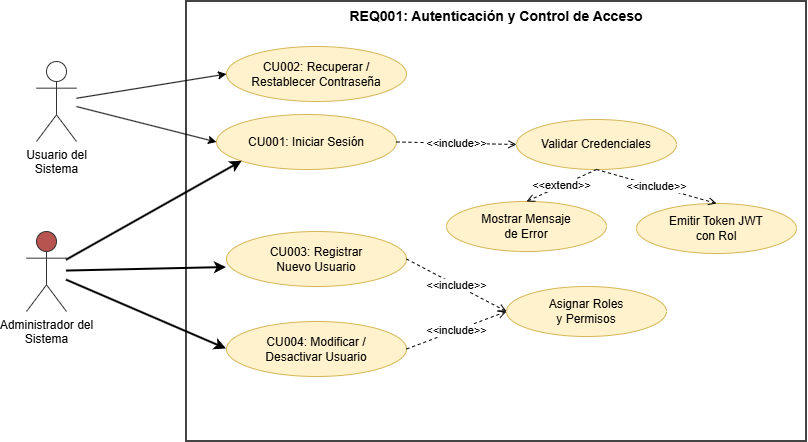
\includegraphics[width=\linewidth]{imagenes/REQ001.png}
\end{figure}

{
\small
\setstretch{1.15}
\setlength{\parindent}{0pt}
\begin{xltabular}{\linewidth}{
    >{\raggedright\arraybackslash}p{3.5cm} 
    >{\raggedright\arraybackslash}X
}
    % --- Encabezado de la primera página ---
    \caption{Especificación del Caso de Uso - REQ001} \label{tab:spec_req001} \\
    \toprule
    \textbf{ID. Req.:} REQ001 & \textbf{ID. Caso de Uso:} CU001 - CU004 \\
    \midrule
    \endfirsthead

    % --- Encabezado en páginas siguientes ---
    \toprule
    \textbf{ID. Req.:} REQ001 & \textbf{ID. Caso de Uso:} CU001 - CU004 \\
    \midrule
    \endhead

    % --- Cierre en página intermedia ---
    \bottomrule
    \endfoot

    % --- Cierre final ---
    \bottomrule
    \endlastfoot

    % --- Filas de contenido ---
    \textbf{Descripción:} & Este caso de uso valida el acceso seguro al sistema mediante credenciales y asigna permisos específicos según el rol. \\
    \midrule
    \textbf{Secuencia Normal:} & 
    1. El usuario ingresa sus credenciales en la pantalla de inicio de sesión. \newline
    2. El sistema valida usuario y contraseña (\textit{si son incorrectos, ver Excepción 1}). \newline
    3. El sistema verifica que la cuenta esté activa (\textit{si está inactiva, ver Excepción 2}). \newline
    4. El sistema genera el token de sesión y aplica el rol autorizado. \newline
    5. El sistema muestra el panel principal con los módulos permitidos. \\
    \midrule
    \textbf{Excepciones:} & 
    \textbf{Excepción 1 (Credenciales incorrectas):} El sistema muestra una advertencia, limpia los campos y retorna al paso 1 de la secuencia normal. \newline
    \textbf{Excepción 2 (Usuario inactivo):} El sistema informa que la cuenta está deshabilitada, finaliza el flujo y conserva al usuario en la pantalla de acceso. \\
\end{xltabular}
}

% ---------------------------------------------------------
% REQ002
% ---------------------------------------------------------
\paragraph{REQ002: Importación y Gestión de Archivos SAT (FEL)}
Describe la carga masiva e importación de facturas electrónicas desde los archivos proporcionados por la SAT (XML/Excel), la extracción de metadatos fiscales y la centralización de comprobantes.


\begin{figure}[H]
    \centering
    \caption{REQ002: Importación y Gestión de Archivos SAT (FEL)}
    \label{fig:REQ002}
    \vspace{0.2cm}
    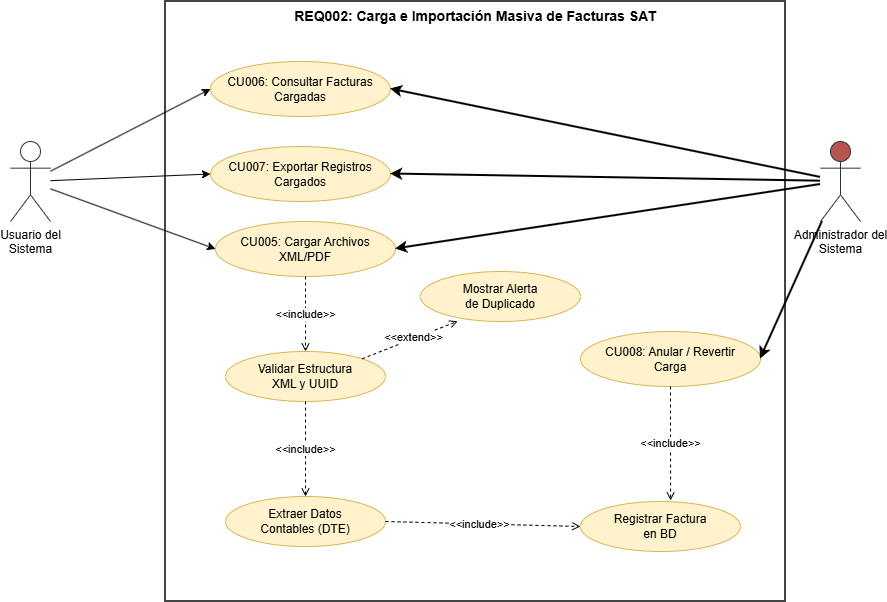
\includegraphics[width=\linewidth]{imagenes/REQ002.png}
\end{figure}

{
\small
\setstretch{1.15}
\setlength{\parindent}{0pt}
\begin{xltabular}{\linewidth}{
    >{\raggedright\arraybackslash}p{3.5cm} 
    >{\raggedright\arraybackslash}X
}
    % --- Encabezado de la primera página ---
    \caption{Especificación del Caso de Uso - REQ002} \label{tab:spec_req002} \\
    \toprule
    \textbf{ID. Req.:} REQ002 & \textbf{ID. Caso de Uso:} CU005 - CU008 \\
    \midrule
    \endfirsthead

    % --- Encabezado en páginas siguientes ---
    \toprule
    \textbf{ID. Req.:} REQ002 & \textbf{ID. Caso de Uso:} CU005 - CU008 \\
    \midrule
    \endhead

    % --- Cierre en página intermedia ---
    \bottomrule
    \endfoot

    % --- Cierre final ---
    \bottomrule
    \endlastfoot

    % --- Filas de contenido ---
    \textbf{Descripción:} & Permite procesar masivamente los reportes mensuales de la SAT, extrayendo metadatos fiscales y centralizando las facturas en la base de datos. \\
    \midrule
    \textbf{Secuencia Normal:} & 
    1. El usuario selecciona y carga el archivo Excel/XML de la SAT (\textit{si el formato no es válido, ver Excepción 1}). \newline
    2. El sistema extrae NIT, nombre, autorización, fecha, monto, IVA y concepto. \newline
    3. El sistema verifica duplicidad y clasifica las facturas (\textit{si existe duplicidad, ver Excepción 2}). \newline
    4. El usuario confirma la carga y el sistema registra las facturas disponibles para Proveedores, Caja chica o Viáticos. \\
    \midrule
    \textbf{Excepciones:} & 
    \textbf{1. Formato no válido:} El sistema informa el error y retorna al paso 1 para seleccionar un archivo válido. \newline
    \textbf{2. Factura duplicada:} El sistema omite el registro, continúa en el paso 2 con la siguiente fila y genera el resumen de omisiones. \newline
    \textbf{3. Concepto no clasificado:} El usuario asigna una cuenta de nomenclatura y el flujo retorna al paso 4. \\
\end{xltabular}
}

% ---------------------------------------------------------
% REQ003
% ---------------------------------------------------------
\paragraph{REQ003: Emisión y Control de Cheques Postfechados}
Ilustra la gestión de cheques emitidos a fecha futura, la asignación de fechas de cobro, el seguimiento de estados (Emitido, Depositado, Anulado) y la programación en calendario.

\begin{figure}[H]
    \centering
    \caption{REQ003: Emisión y Control de Cheques Postfechados}
    \label{fig:REQ003}
    \vspace{0.2cm}
    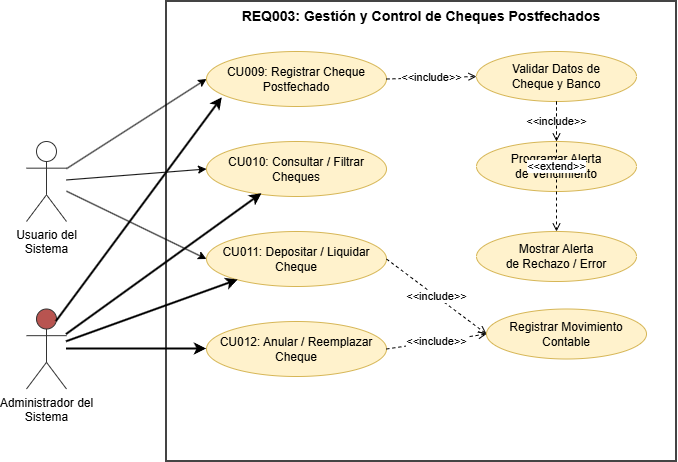
\includegraphics[width=\linewidth]{imagenes/REQ003.png}
\end{figure}

{
\small
\setstretch{1.15}
\setlength{\parindent}{0pt}
\begin{xltabular}{\linewidth}{
    >{\raggedright\arraybackslash}p{3.5cm} 
    >{\raggedright\arraybackslash}X
}
    % --- Encabezado de la primera página ---
    \caption{Especificación del Caso de Uso - REQ003} \label{tab:spec_req003} \\
    \toprule
    \textbf{ID. Req.:} REQ003 & \textbf{ID. Caso de Uso:} CU009 - CU012 \\
    \midrule
    \endfirsthead

    % --- Encabezado en páginas siguientes ---
    \toprule
    \textbf{ID. Req.:} REQ003 & \textbf{ID. Caso de Uso:} CU009 - CU012 \\
    \midrule
    \endhead

    % --- Cierre en página intermedia ---
    \bottomrule
    \endfoot

    % --- Cierre final ---
    \bottomrule
    \endlastfoot

    % --- Filas de contenido ---
    \textbf{Descripción:} & Automatiza el control de cheques recibidos/emitidos con fecha posterior, ajustando sus fechas de depósito a días hábiles. \\
    \midrule
    \textbf{Secuencia Normal:} & 
    1. El usuario registra cliente, banco del cheque, banco de depósito, número, monto y fechas (\textit{si faltan datos, ver Excepción 1}). \newline
    2. El sistema verifica que el número de cheque no esté registrado (\textit{si existe, ver Excepción 1}). \newline
    3. El sistema asigna estado Pendiente y ajusta la fecha de depósito a un día hábil. \newline
    4. El sistema guarda el cheque y lo incorpora al calendario (\textit{si es rechazado, ver Excepción 2}). \\
    \midrule
    \textbf{Excepciones:} & 
    \textbf{1. Cheque duplicado o incompleto:} El sistema informa el problema y retorna al paso 1 para corregir los datos. \newline
    \textbf{2. Cheque rechazado:} El usuario registra recepción del rechazo y una nueva fecha; el flujo retorna al paso 4 para actualizar el calendario. \\
\end{xltabular}
}

% ---------------------------------------------------------
% REQ004
% ---------------------------------------------------------
\paragraph{REQ004: Creación y Control de Fondo de Caja Chica}
Aborda la asignación de facturas SAT y comprobantes no fiscales (vales/recibos), la ejecución de cálculos contables automatizados y la generación de borradores de partidas de diario.

\begin{figure}[H]
    \centering
    \caption{REQ004: Creación y Control de Fondo de Caja Chica}
    \label{fig:REQ004}
    \vspace{0.2cm}
    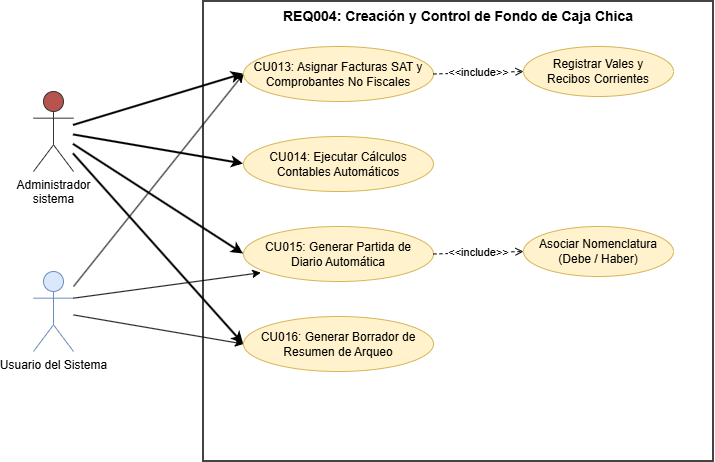
\includegraphics[width=\linewidth]{imagenes/REQ004.png}
\end{figure}

{
\small
\setstretch{1.15}
\setlength{\parindent}{0pt}
\begin{xltabular}{\linewidth}{
    >{\raggedright\arraybackslash}p{3.5cm} 
    >{\raggedright\arraybackslash}X
}
    % --- Encabezado de la primera página ---
    \caption{Especificación del Caso de Uso - REQ004} \label{tab:spec_req004} \\
    \toprule
    \textbf{ID. Req.:} REQ004 & \textbf{ID. Caso de Uso:} CU013 - CU016 \\
    \midrule
    \endfirsthead

    % --- Encabezado en páginas siguientes ---
    \toprule
    \textbf{ID. Req.:} REQ004 & \textbf{ID. Caso de Uso:} CU013 - CU016 \\
    \midrule
    \endhead

    % --- Cierre en página intermedia ---
    \bottomrule
    \endfoot

    % --- Cierre final ---
    \bottomrule
    \endlastfoot

    % --- Filas de contenido ---
    \textbf{Descripción:} & Gestiona los desembolsos de caja chica agrupando comprobantes fiscales y vales internos, generando partidas automáticas. \\
    \midrule
    \textbf{Secuencia Normal:} & 
    1. El auxiliar llama una factura FEL por número o registra un Recibo/otro documento. \newline
    2. El sistema muestra el movimiento y propone una cuenta de nomenclatura (\textit{si no reconoce el concepto, ver Excepción 1}). \newline
    3. El usuario confirma o asigna la cuenta contable y el sistema calcula gastos, IVA y total. \newline
    4. El sistema genera la partida contable y el resumen imprimible de Caja chica. \\
    \midrule
    \textbf{Excepciones:} & 
    \textbf{1. Factura asignada a otro módulo:} El sistema informa el bloqueo y retorna al paso 1 para seleccionar otro comprobante. \newline
    \textbf{2. Cuenta no reconocida:} Se despliega el selector de nomenclatura; al elegir una cuenta, el flujo retorna al paso 3. \newline
    \textbf{3. Debe y Haber descuadrados:} El sistema detiene la generación y retorna al paso 3 para corregir la cuenta o el monto. \\
\end{xltabular}
}

% ---------------------------------------------------------
% REQ005
% ---------------------------------------------------------
\paragraph{REQ005: Liquidación y Reintegro de Viáticos}
Muestra el flujo de asociación de facturas físicas por colaborador mediante número correlativo, la programación de giras organizadas por semanas calendario y el cálculo de reembolsos.


\begin{figure}[H]
    \centering
    \caption{REQ005: Liquidación y Reintegro de Viáticos}
    \label{fig:REQ005}
    \vspace{0.2cm}
    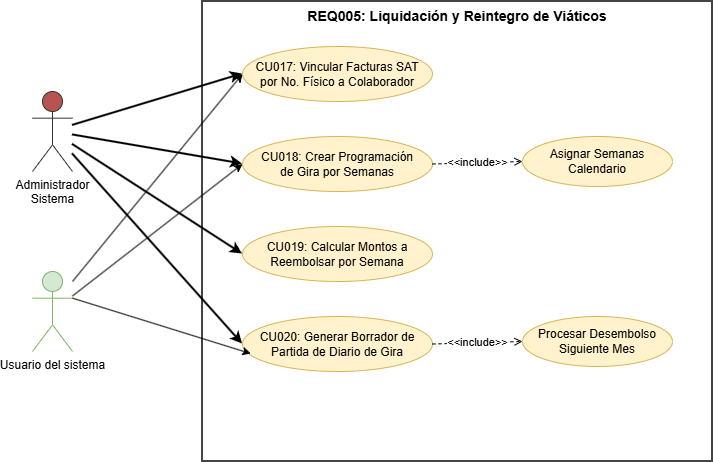
\includegraphics[width=\linewidth]{imagenes/REQ005.png}
\end{figure}

{
\small
\setstretch{1.15}
\setlength{\parindent}{0pt}
\begin{xltabular}{\linewidth}{
    >{\raggedright\arraybackslash}p{3.5cm} 
    >{\raggedright\arraybackslash}X
}
    % --- Encabezado de la primera página ---
    \caption{Especificación del Caso de Uso - REQ005} \label{tab:spec_req005} \\
    \toprule
    \textbf{ID. Req.:} REQ005 & \textbf{ID. Caso de Uso:} CU017 - CU020 \\
    \midrule
    \endfirsthead

    % --- Encabezado en páginas siguientes ---
    \toprule
    \textbf{ID. Req.:} REQ005 & \textbf{ID. Caso de Uso:} CU017 - CU020 \\
    \midrule
    \endhead

    % --- Cierre en página intermedia ---
    \bottomrule
    \endfoot

    % --- Cierre final ---
    \bottomrule
    \endlastfoot

    % --- Filas de contenido ---
    \textbf{Descripción:} & Controla las liquidaciones de viáticos de los colaboradores, vinculando sus facturas entregadas con la programación de giras. \\
    \midrule
    \textbf{Secuencia Normal:} & 
    1. El usuario selecciona colaborador, territorio y semana de gira 1 a 5. \newline
    2. El usuario asigna facturas por número a Viáticos, Movilidad, Actividades o Bonos/otros gastos (\textit{si no se reconoce la cuenta, ver Excepción 1}). \newline
    3. El sistema calcula los gastos de la liquidación y aplica la regla de Movilidad de la primera semana. \newline
    4. El sistema genera la partida semanal o transitoria según la fecha y el estado de reintegro. \\
    \midrule
    \textbf{Excepciones:} & 
    \textbf{1. Factura no encontrada:} El sistema informa el resultado y retorna al paso 2 para buscar otro número o cargar la factura. \newline
    \textbf{2. Factura asignada a otro módulo:} Se bloquea la vinculación y el flujo retorna al paso 2 para seleccionar otro comprobante. \newline
    \textbf{3. Semana no válida para Movilidad:} El sistema informa que Movilidad corresponde a la semana 1 y retorna al paso 1. \\
\end{xltabular}
}

% ---------------------------------------------------------
% REQ006
% ---------------------------------------------------------
\paragraph{REQ006: Programación de Pagos a Proveedores}
Establece la gestión de la ficha del proveedor (días de crédito y retenciones IVA/ISR), la vinculación con facturas de la SAT y el cálculo automático de fechas de vencimiento.


\begin{figure}[H]
    \centering
    \caption{REQ006: Programación de Pagos a Proveedores}
    \label{fig:REQ006}
    \vspace{0.2cm}
    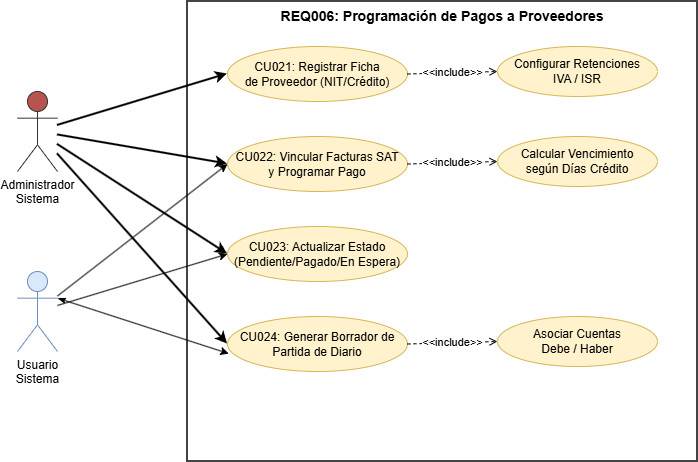
\includegraphics[width=\linewidth]{imagenes/REQ006.png}
\end{figure}

{
\small
\setstretch{1.15}
\setlength{\parindent}{0pt}
\begin{xltabular}{\linewidth}{
    >{\raggedright\arraybackslash}p{3.5cm} 
    >{\raggedright\arraybackslash}X
}
    % --- Encabezado de la primera página ---
    \caption{Especificación del Caso de Uso - REQ006} \label{tab:spec_req006} \\
    \toprule
    \textbf{ID. Req.:} REQ006 & \textbf{ID. Caso de Uso:} CU021 - CU024 \\
    \midrule
    \endfirsthead

    % --- Encabezado en páginas siguientes ---
    \toprule
    \textbf{ID. Req.:} REQ006 & \textbf{ID. Caso de Uso:} CU021 - CU024 \\
    \midrule
    \endhead

    % --- Cierre en página intermedia ---
    \bottomrule
    \endfoot

    % --- Cierre final ---
    \bottomrule
    \endlastfoot

    % --- Filas de contenido ---
    \textbf{Descripción:} & Administra los compromisos comerciales con proveedores a crédito, calculando vencimientos y reteniendo impuestos según ley. \\
    \midrule
    \textbf{Secuencia Normal:} & 
    1. El usuario registra NIT, días de crédito, retenciones y cuenta de nomenclatura del proveedor. \newline
    2. El sistema completa los nombres y despliega las facturas del proveedor por mes. \newline
    3. El sistema calcula vencimiento, retenciones y descuentos (\textit{si el vencimiento cruza el mes, ver Excepción 2}). \newline
    4. El usuario genera la partida dentro del mes o la partida transitoria con gastos e IVA en Debe y retenciones/descuentos en Haber. \\
    \midrule
    \textbf{Excepciones:} & 
    \textbf{1. Proveedor no registrado:} El sistema solicita crear la ficha y retorna al paso 1. \newline
    \textbf{2. Factura previamente pagada o anulada:} El sistema bloquea el procesamiento y retorna al paso 2 para seleccionar otra factura. \newline
    \textbf{3. Vencimiento fuera del mes:} El sistema dirige la factura a Cuenta transitoria y retorna al paso 4 para generar la partida correspondiente. \\
\end{xltabular}
}

% ---------------------------------------------------------
% REQ007
% ---------------------------------------------------------
\paragraph{REQ007: Módulo de Calendario Dinámico y Programación Operativa}
Consolida en una interfaz visual e interactiva las fechas de cobro de cheques, vencimientos de proveedores y liquidaciones de viáticos, permitiendo reprogramaciones en tiempo real.

\begin{figure}[H]
    \centering
    \caption{REQ007: Módulo de Calendario Dinámico y Programación Operativa}
    \label{fig:REQ007}
    \vspace{0.2cm}
    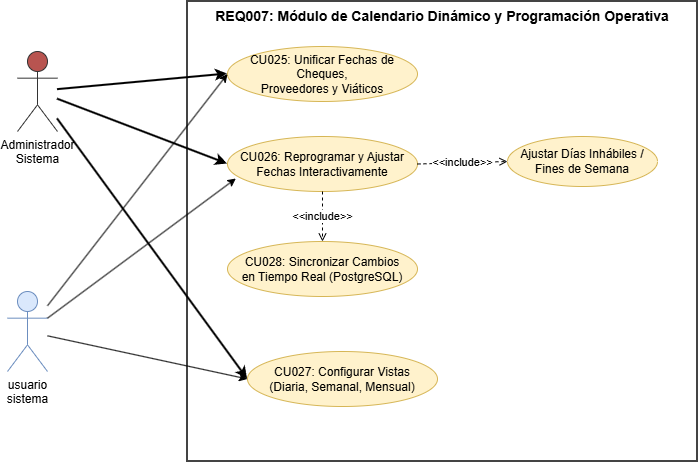
\includegraphics[width=\linewidth]{imagenes/REQ007.png}
\end{figure}

{
\small
\setstretch{1.15}
\setlength{\parindent}{0pt}
\begin{xltabular}{\linewidth}{
    >{\raggedright\arraybackslash}p{3.5cm} 
    >{\raggedright\arraybackslash}X
}
    % --- Encabezado de la primera página ---
    \caption{Especificación del Caso de Uso - REQ007} \label{tab:spec_req007} \\
    \toprule
    \textbf{ID. Req.:} REQ007 & \textbf{ID. Caso de Uso:} CU025 - CU028 \\
    \midrule
    \endfirsthead

    % --- Encabezado en páginas siguientes ---
    \toprule
    \textbf{ID. Req.:} REQ007 & \textbf{ID. Caso de Uso:} CU025 - CU028 \\
    \midrule
    \endhead

    % --- Cierre en página intermedia ---
    \bottomrule
    \endfoot

    % --- Cierre final ---
    \bottomrule
    \endlastfoot

    % --- Filas de contenido ---
    \textbf{Descripción:} & Ofrece una vista consolidada de los compromisos contables del mes con capacidad de edición directa mediante interfaz gráfica. \\
    \midrule
    \textbf{Secuencia Normal:} & 
    1. El sistema recupera las actividades de cheques, proveedores y viáticos. \newline
    2. El usuario consulta la agenda en vista mensual, semanal o diaria. \newline
    3. El usuario selecciona una actividad y solicita reprogramación (\textit{si cae en día inhábil, ver Excepción 1}). \newline
    4. El sistema guarda la nueva fecha y actualiza la vista del calendario. \\
    \midrule
    \textbf{Excepciones:} & 
    \textbf{1. Reprogramación en día inhábil:} El sistema propone el día hábil más cercano y retorna al paso 3 para confirmar. \newline
    \textbf{2. Error de conexión:} Se informa el error, se conserva la fecha anterior y se retorna al paso 3 para reintentar. \newline
    \textbf{3. Sin actividad registrada:} El sistema muestra el calendario vacío y retorna al paso 1 para ajustar el período. \\
\end{xltabular}
}

% ---------------------------------------------------------
% REQ008
% ---------------------------------------------------------
\paragraph{REQ008: Nomenclatura Contable y Partidas Automáticas}
Detalla la estructura del catálogo de cuentas contables, la parametrización de reglas para el Debe y el Haber, y la construcción del borrador de la partida contable.

\begin{figure}[H]
    \centering
    \caption{REQ008: Nomenclatura Contable y Partidas Automáticas}
    \label{fig:REQ008}
    \vspace{0.2cm}
    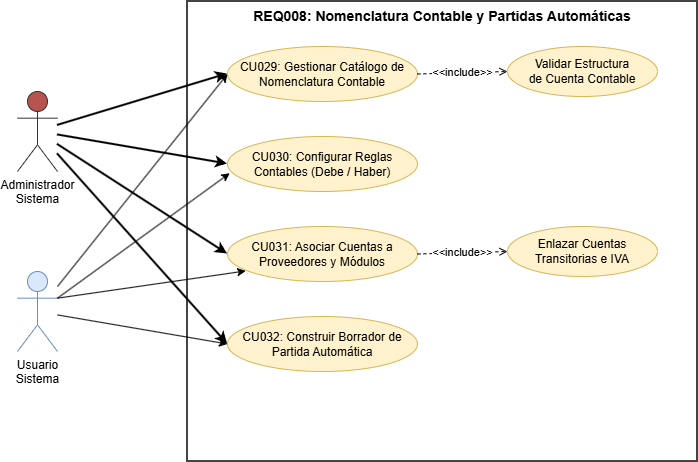
\includegraphics[width=\linewidth]{imagenes/REQ008.png}
\end{figure}

{
\small
\setstretch{1.15}
\setlength{\parindent}{0pt}
\begin{xltabular}{\linewidth}{
    >{\raggedright\arraybackslash}p{3.5cm} 
    >{\raggedright\arraybackslash}X
}
    % --- Encabezado de la primera página ---
    \caption{Especificación del Caso de Uso - REQ008} \label{tab:spec_req008} \\
    \toprule
    \textbf{ID. Req.:} REQ008 & \textbf{ID. Caso de Uso:} CU029 - CU032 \\
    \midrule
    \endfirsthead

    % --- Encabezado en páginas siguientes ---
    \toprule
    \textbf{ID. Req.:} REQ008 & \textbf{ID. Caso de Uso:} CU029 - CU032 \\
    \midrule
    \endhead

    % --- Cierre en página intermedia ---
    \bottomrule
    \endfoot

    % --- Cierre final ---
    \bottomrule
    \endlastfoot

    % --- Filas de contenido ---
    \textbf{Descripción:} & Define la parametrización contable del sistema garantizando la correcta generación de asientos balanceados. \\
    \midrule
    \textbf{Secuencia Normal:} & 
    1. El administrador registra una cuenta con código, nombre y naturaleza Debe o Haber (\textit{si el código existe, ver Excepción 1}). \newline
    2. El sistema muestra la cuenta activa en el catálogo y la ofrece en los selectores de clasificación. \newline
    3. El usuario asigna cuentas a proveedores, Caja chica o Viáticos. \newline
    4. El sistema genera la partida y verifica que Debe y Haber coincidan (\textit{si no coinciden, ver Excepción 2}). \\
    \midrule
    \textbf{Excepciones:} & 
    \textbf{1. Código duplicado:} Se bloquea el guardado y el flujo retorna al paso 1 para ingresar otro código. \newline
    \textbf{2. Partida descuadrada (Debe $\neq$ Haber):} El sistema resalta la diferencia y retorna al paso 4 para corregir la clasificación. \newline
    \textbf{3. Cuenta inactiva:} El selector la excluye y el flujo retorna al paso 2 para elegir una cuenta activa. \\
\end{xltabular}
}

% ---------------------------------------------------------
% REQ009
% ---------------------------------------------------------
\paragraph{REQ009: Generación de Reportes Operativos y Financieros}
Contempla la extracción y consolidación de reportes de cheques postfechados, proyecciones a proveedores, arqueos de caja chica y gastos de viáticos por colaborador.

\begin{figure}[H]
    \centering
    \caption{REQ009: Generación de Reportes Operativos y Financieros}
    \label{fig:REQ009}
    \vspace{0.2cm}
    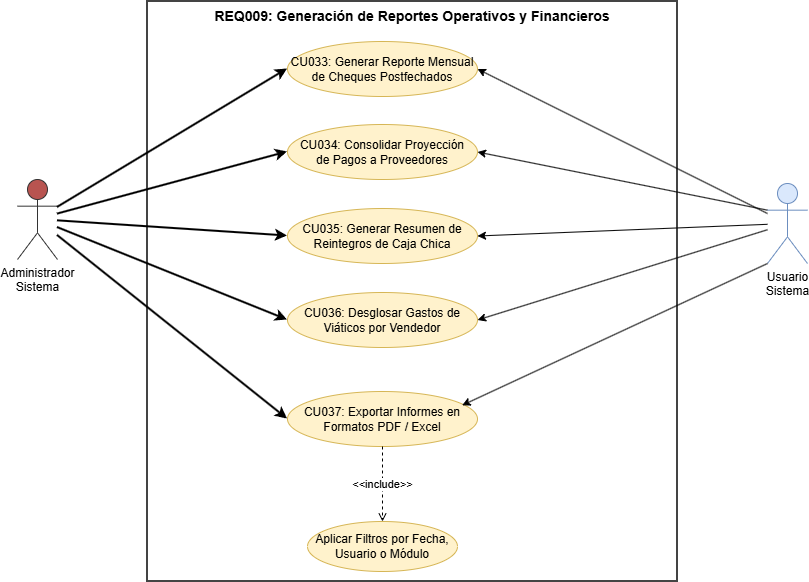
\includegraphics[width=\linewidth]{imagenes/REQ009.png}
\end{figure}

{
\small
\setstretch{1.15}
\setlength{\parindent}{0pt}
\begin{xltabular}{\linewidth}{
    >{\raggedright\arraybackslash}p{3.5cm} 
    >{\raggedright\arraybackslash}X
}
    % --- Encabezado de la primera página ---
    \caption{Especificación del Caso de Uso - REQ009} \label{tab:spec_req009} \\
    \toprule
    \textbf{ID. Req.:} REQ009 & \textbf{ID. Caso de Uso:} CU033 - CU037 \\
    \midrule
    \endfirsthead

    % --- Encabezado en páginas siguientes ---
    \toprule
    \textbf{ID. Req.:} REQ009 & \textbf{ID. Caso de Uso:} CU033 - CU037 \\
    \midrule
    \endhead

    % --- Cierre en página intermedia ---
    \bottomrule
    \endfoot

    % --- Cierre final ---
    \bottomrule
    \endlastfoot

    % --- Filas de contenido ---
    \textbf{Descripción:} & Permite consultar y exportar resúmenes financieros y operativos filtrados por rangos de fechas o entidades. \\
    \midrule
    \textbf{Secuencia Normal:} & 
    1. El usuario selecciona el tipo de reporte y sus filtros (\textit{si no hay registros, ver Excepción 1}). \newline
    2. El sistema consulta y consolida la información de los módulos. \newline
    3. El usuario revisa la vista previa. \newline
    4. El usuario imprime o exporta el resultado (\textit{si falla la exportación, ver Excepción 2}). \\
    \midrule
    \textbf{Excepciones:} & 
    \textbf{1. Sin datos en el rango seleccionado:} El sistema informa la ausencia de registros y retorna al paso 1 para cambiar los filtros. \newline
    \textbf{2. Error de exportación:} Se informa el fallo y retorna al paso 4 para reintentar la impresión o exportación. \\
\end{xltabular}
}


\subsubsection{Base de Datos}
El diseño relacional para la base de datos PostgreSQL integra la estructura de tablas, tipos enumerados y restricciones de claves foráneas requeridas para garantizar la integridad referencial de los módulos del sistema.

\begin{figure}[H]
    \centering
    \caption{Diagrama de Base de Datos Relacional}
    \label{fig:diagramabd}
    \vspace{0.2cm}
    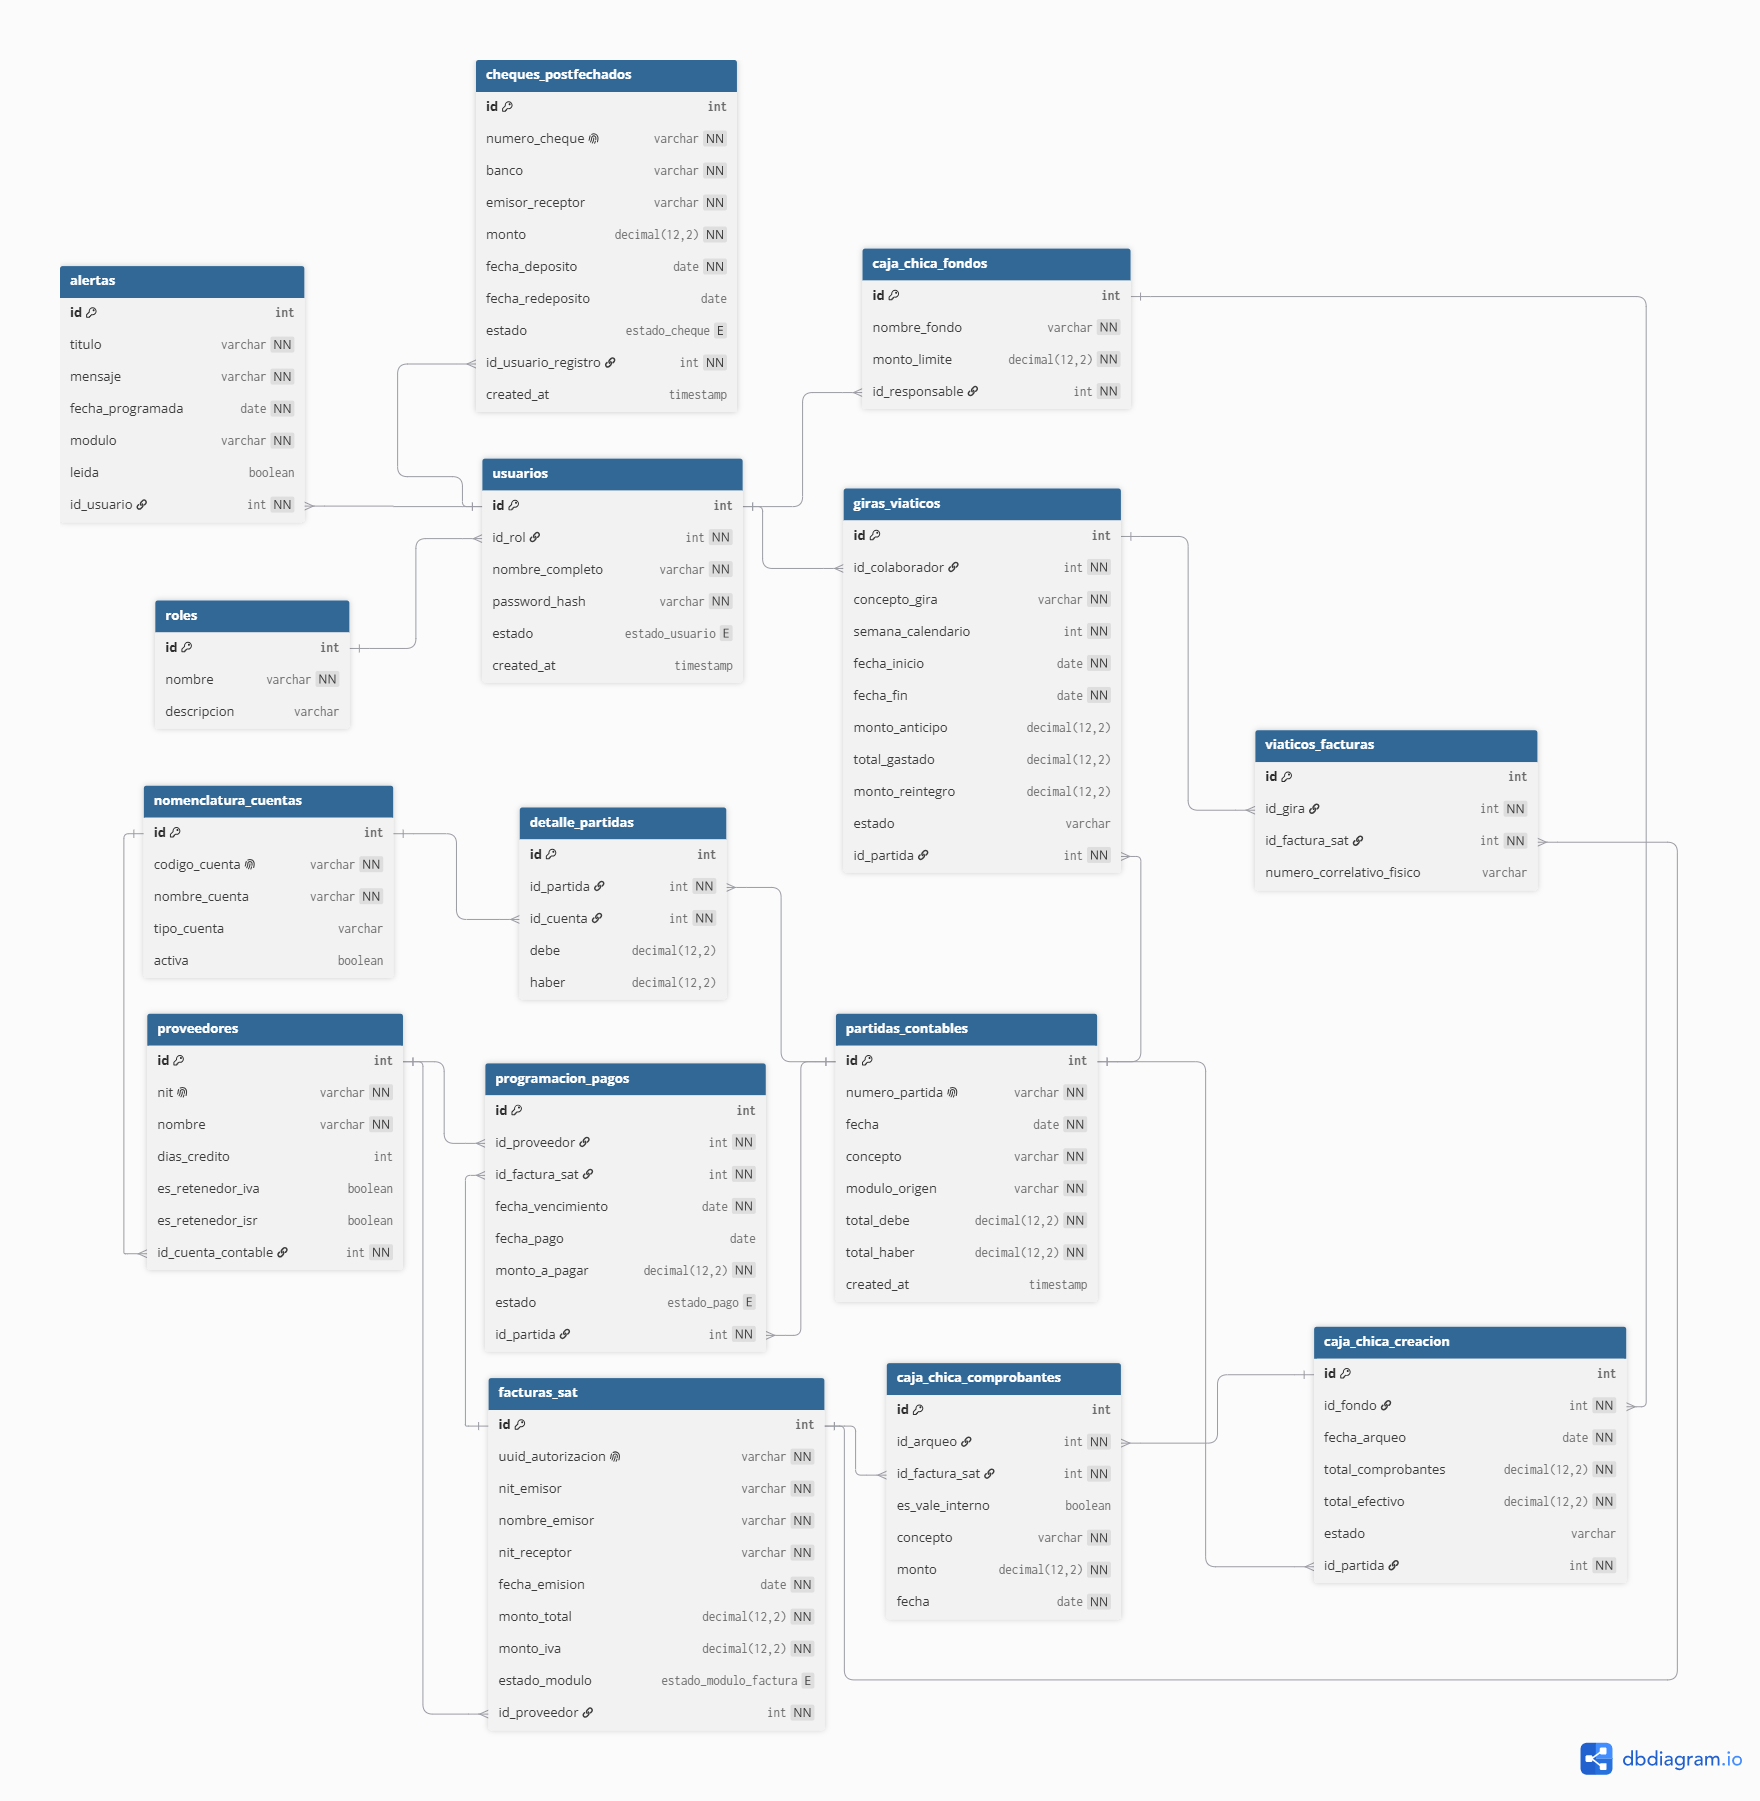
\includegraphics[width=\linewidth, height=\textheight, keepaspectratio]{imagenes/diagramabd.png}
    \vspace{0.2cm}
   
\end{figure}

\subsection{Diseño de Elementos}

La sección presenta los diseños visuales del Sistema Web y registra sus controles reutilizables. Las figuras se organizan por pantalla y por tipo de componente, evitando repetir nombres de botones o controles que aparecen en más de un módulo.

\subsubsection{Componentes visuales agrupados}

\begin{figure}[H]
    \centering
    \caption{Botones y acciones reutilizables del Sistema Web}
    \label{fig:componentes_botones}
    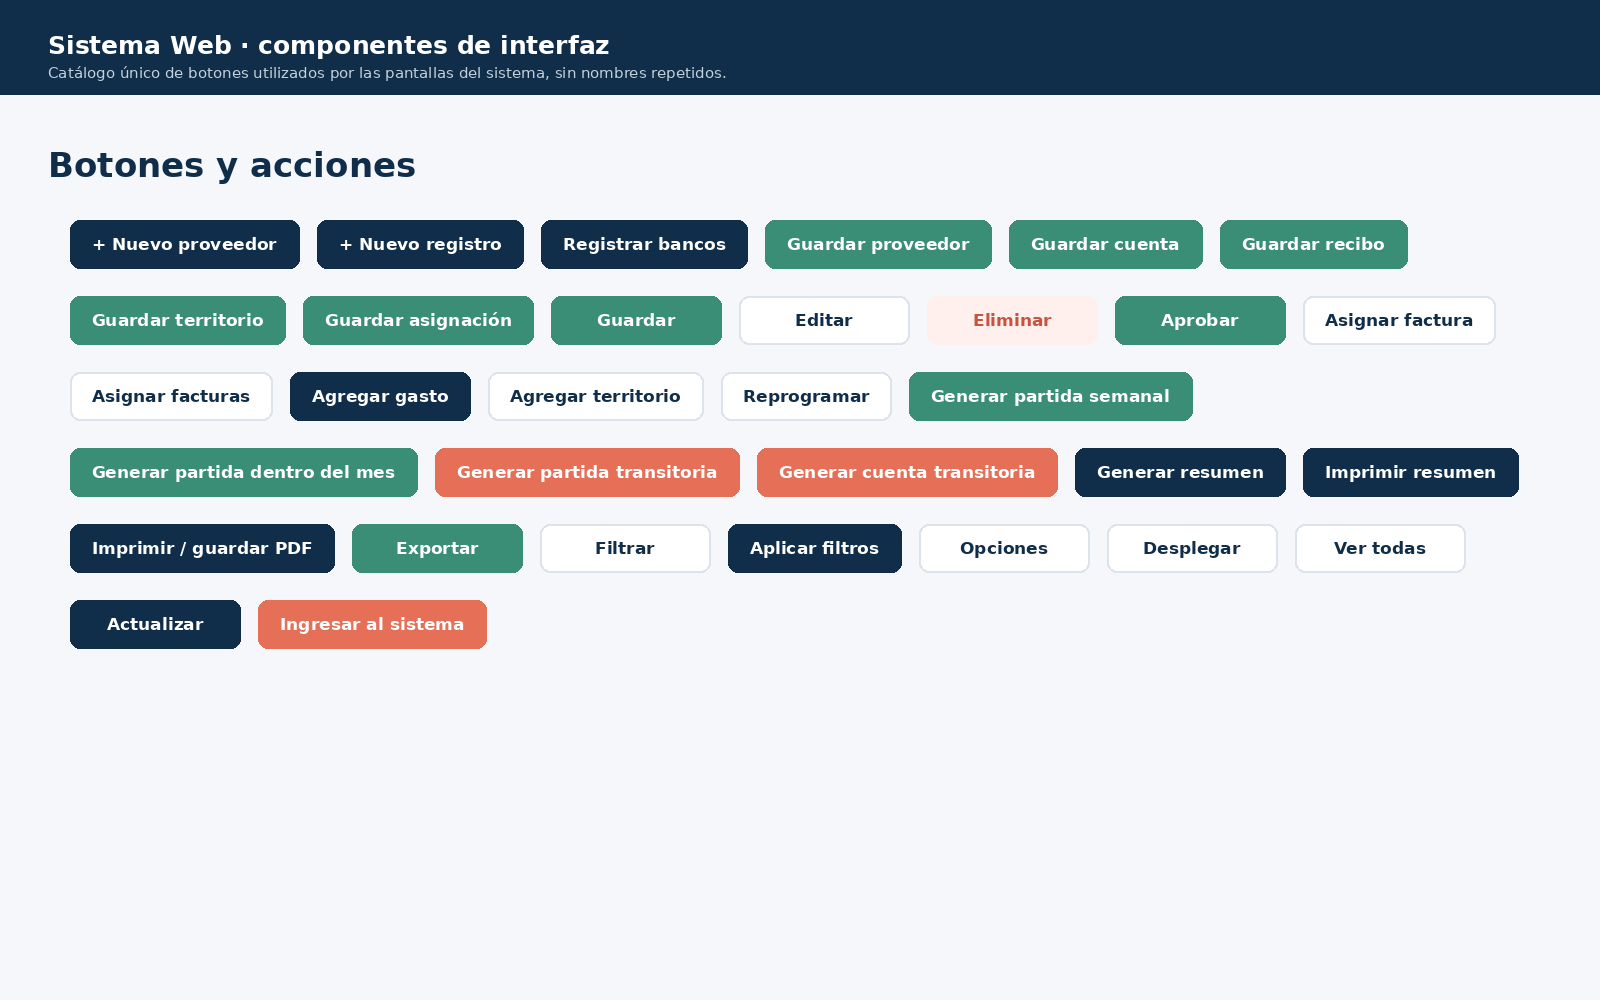
\includegraphics[width=0.96\linewidth]{imagenes/elementos_01_botones.png}
\end{figure}

\begin{figure}[H]
    \centering
    \caption{Listas desplegables y opciones de selección}
    \label{fig:componentes_listas}
    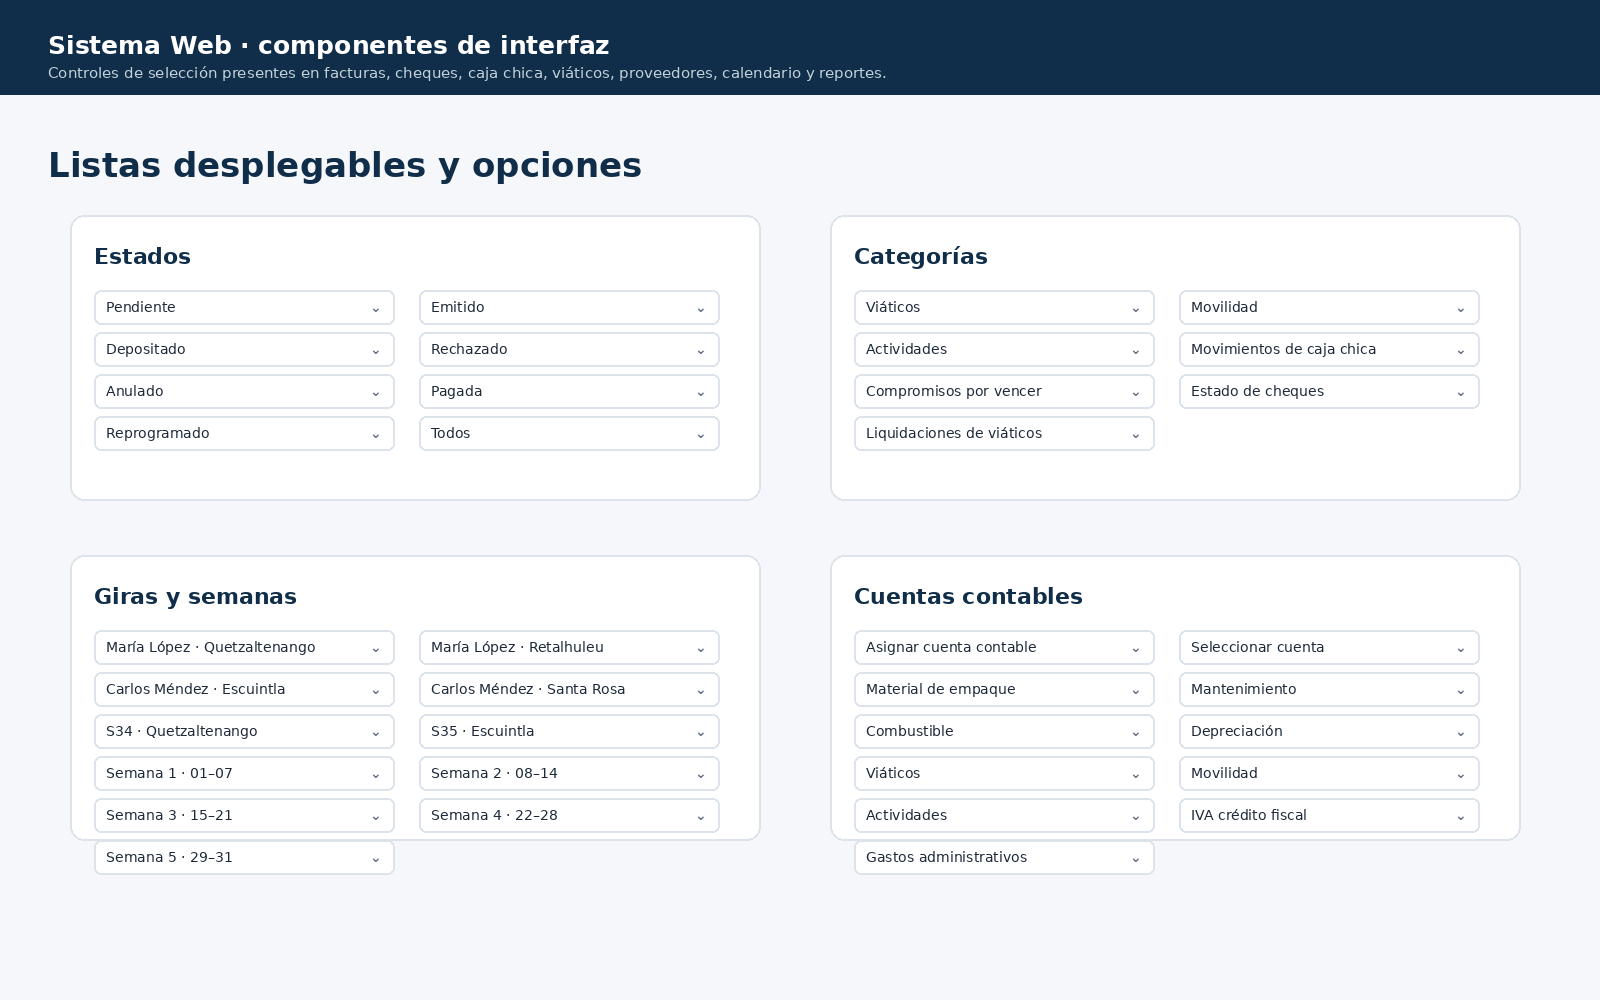
\includegraphics[width=0.96\linewidth]{imagenes/elementos_02_listas_desplegables.png}
\end{figure}

\begin{figure}[H]
    \centering
    \caption{Formularios y campos de captura}
    \label{fig:componentes_formularios}
    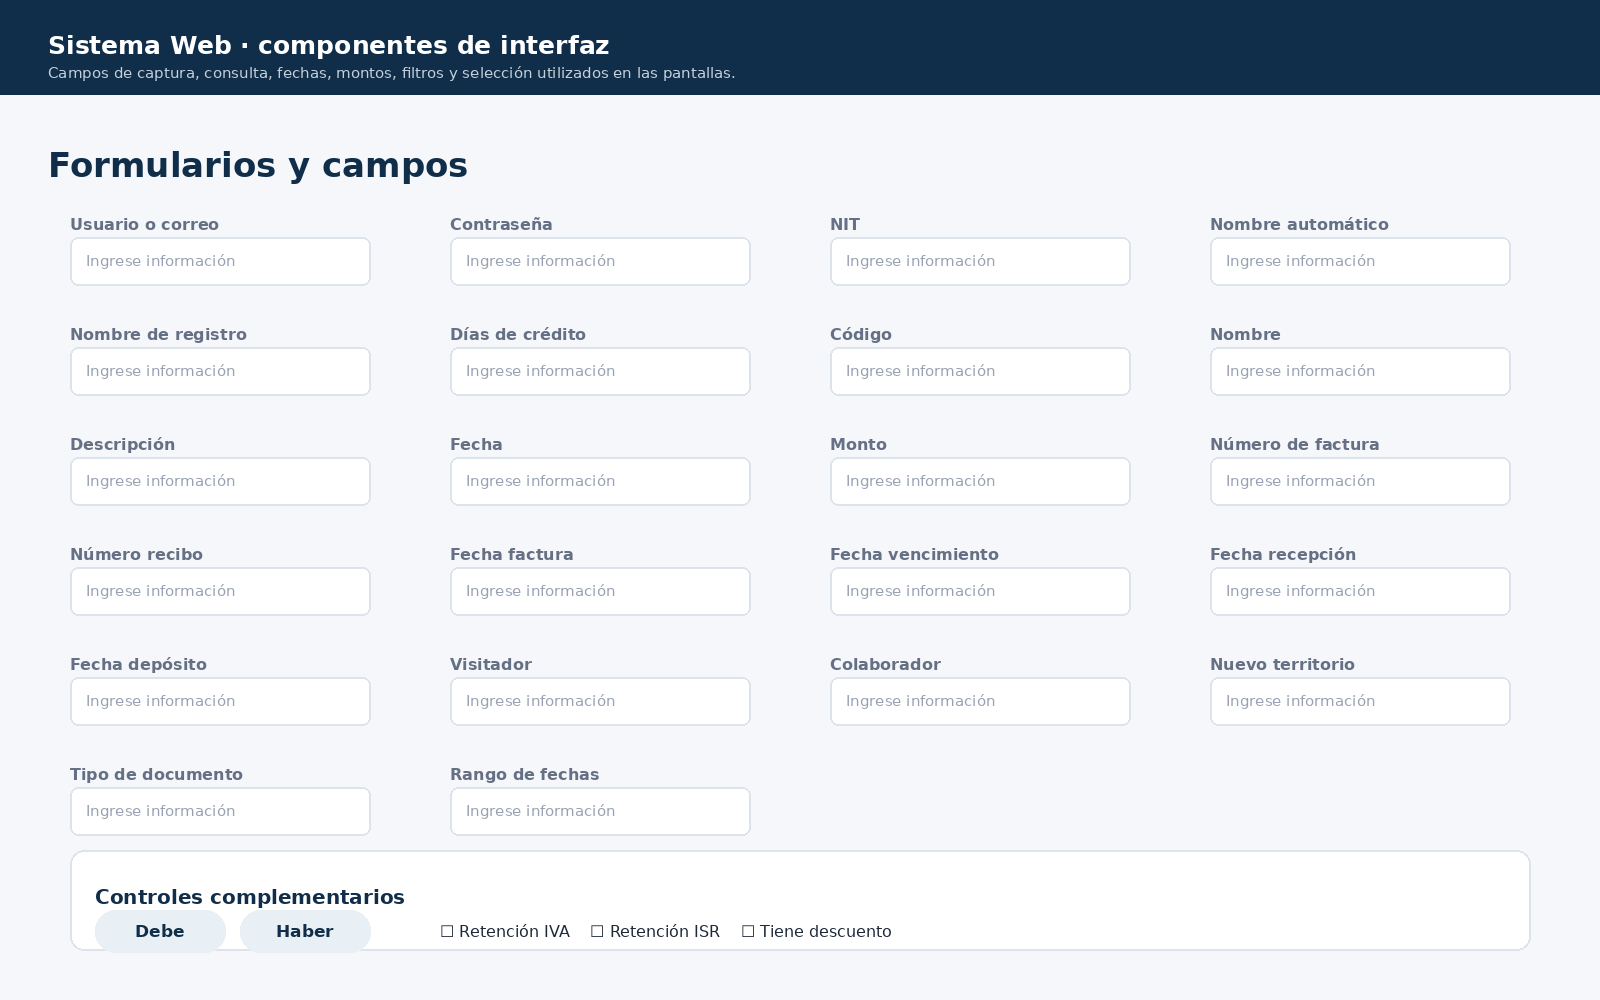
\includegraphics[width=0.96\linewidth]{imagenes/elementos_03_formularios.png}
\end{figure}

\begin{figure}[H]
    \centering
    \caption{Tablas, tarjetas y estados operativos}
    \label{fig:componentes_tablas}
    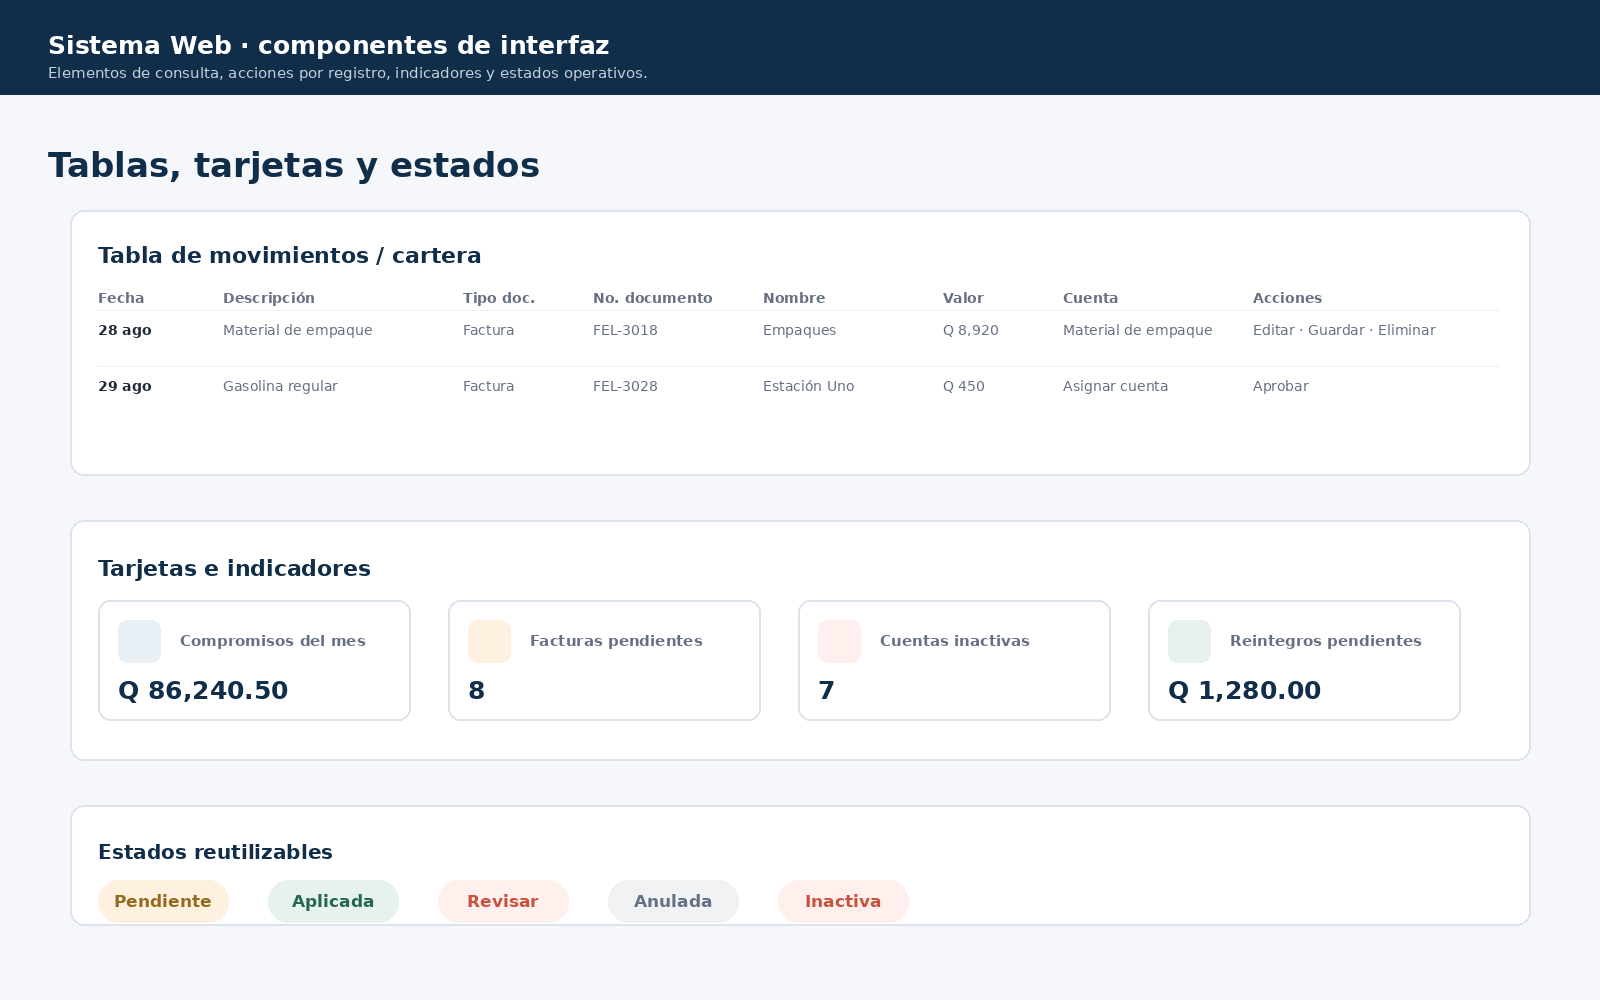
\includegraphics[width=0.96\linewidth]{imagenes/elementos_04_tablas_tarjetas.png}
\end{figure}

\begin{figure}[H]
    \centering
    \caption{Acciones contables, generación e impresión}
    \label{fig:componentes_contables}
    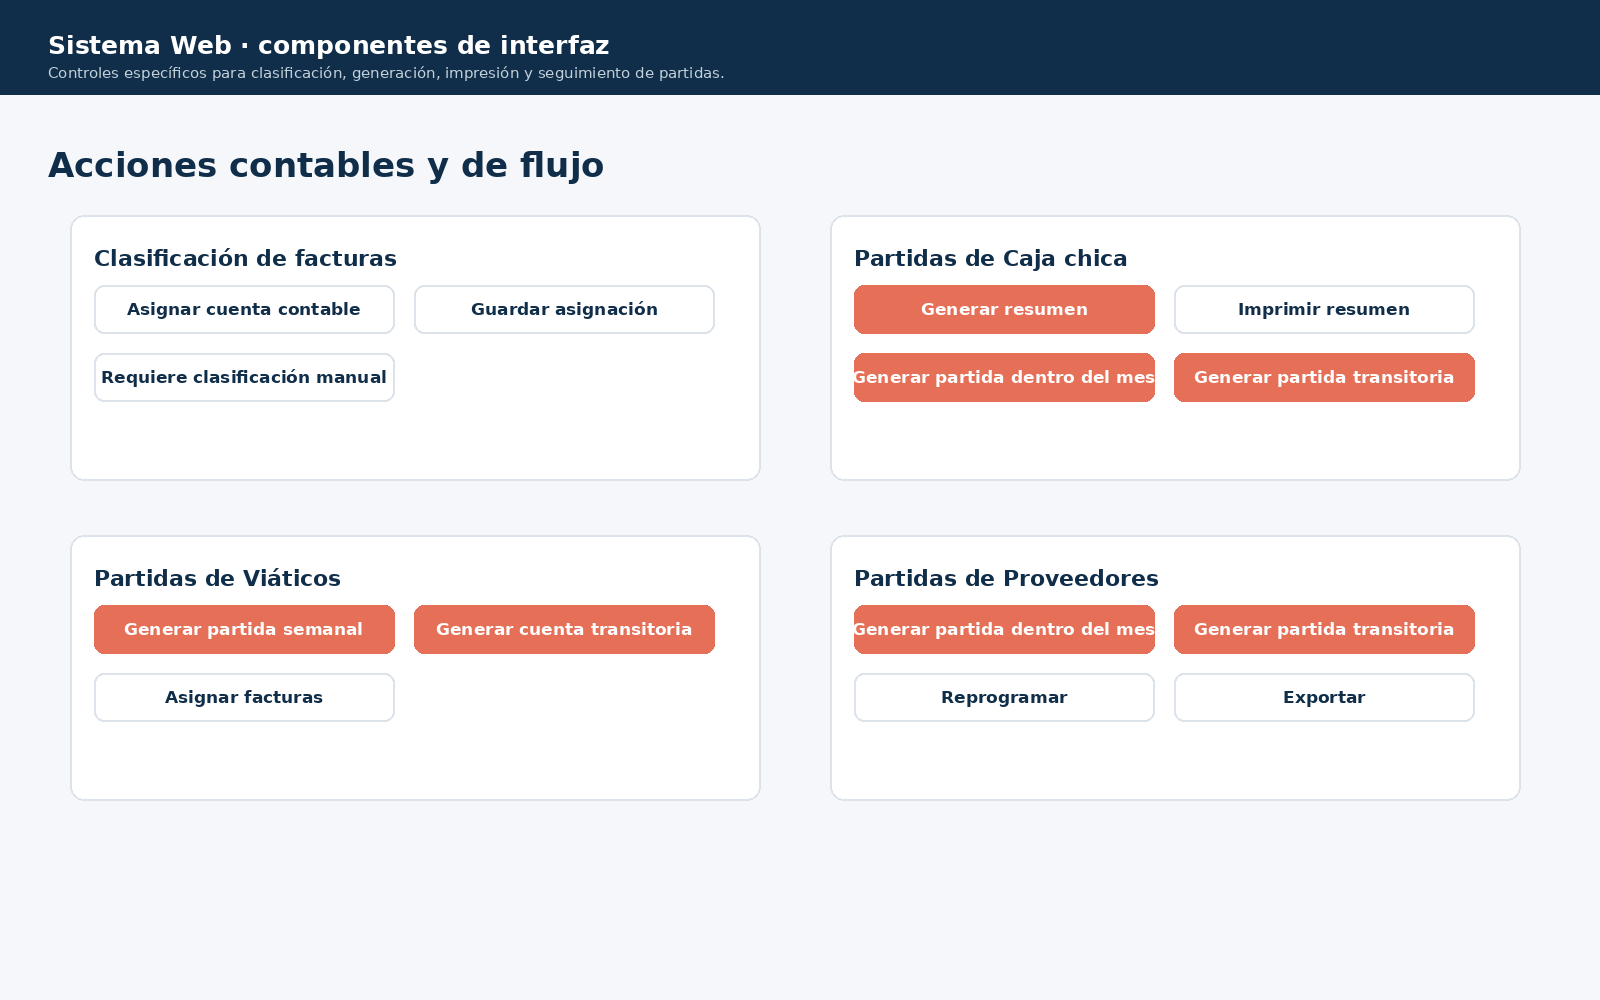
\includegraphics[width=0.96\linewidth]{imagenes/elementos_05_acciones_contables.png}
\end{figure}

\subsubsection{Diseños visuales individuales del sistema}

\begin{figure}[H]
    \centering
    \caption{Pantalla de inicio de sesión}
    \label{fig:pantalla_login}
    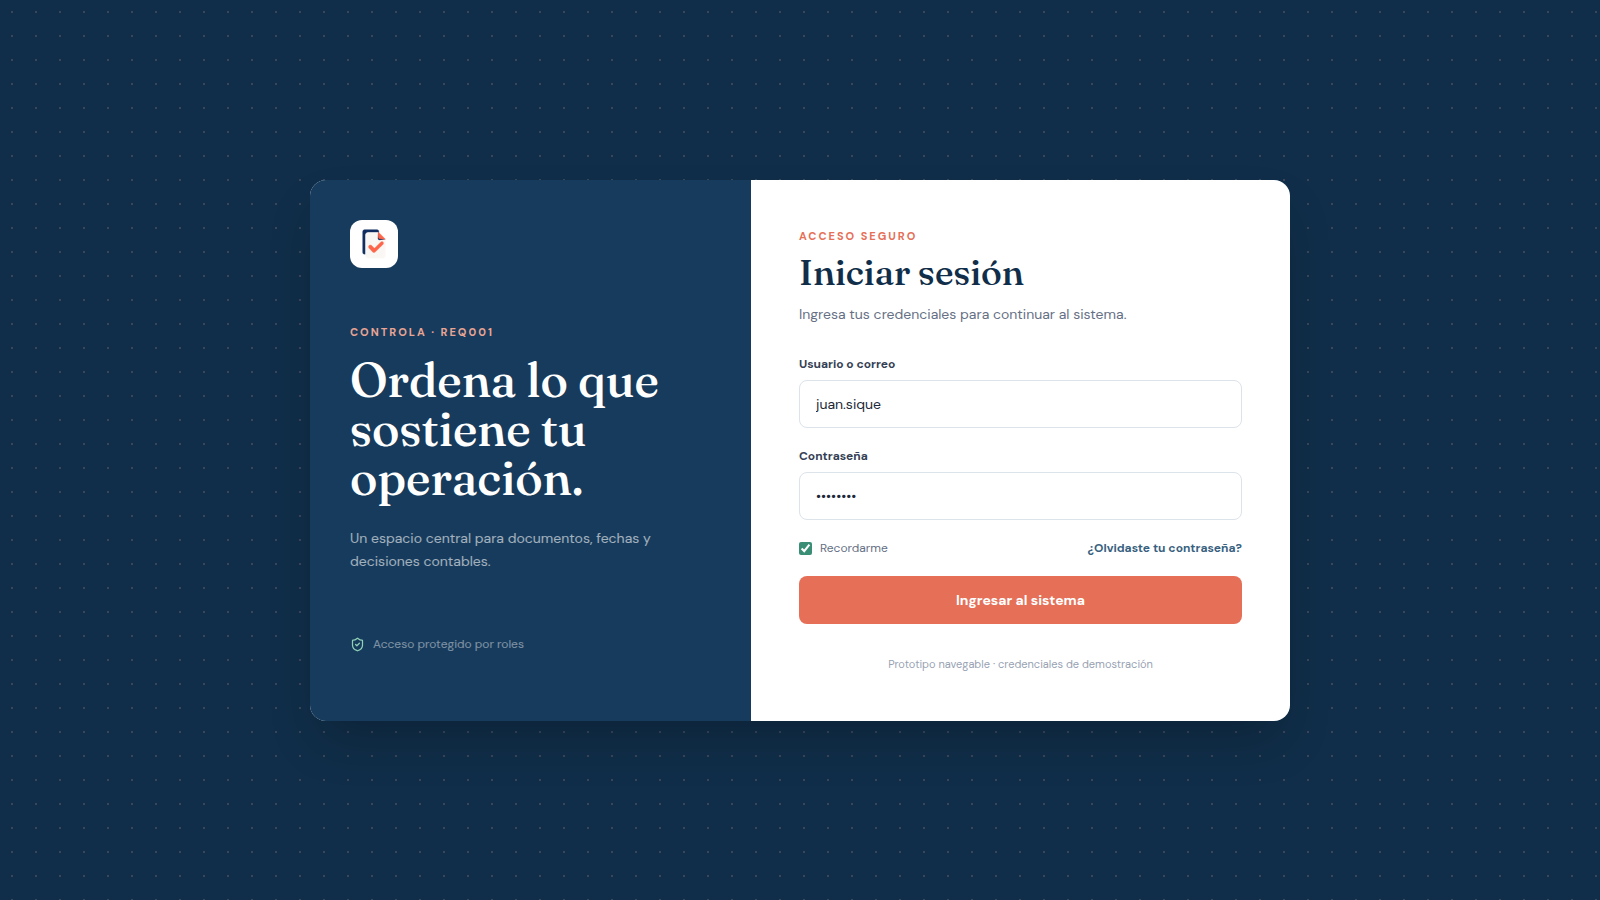
\includegraphics[width=0.96\linewidth]{imagenes/pantalla_01_login.png}
\end{figure}
\begin{table}[H]\centering
\caption{Descripción de Campos de la Pantalla de Autenticación de Usuarios}
\label{tab:3_12_pantalla_login}
\small\setstretch{1.15}
\begin{tabular}{p{0.25\linewidth}p{0.20\linewidth}p{0.20\linewidth}p{0.27\linewidth}}
\toprule
\textbf{Campo o control} & \textbf{Tipo} & \textbf{Valor por defecto} & \textbf{Observación} \\
\midrule
Usuario o correo & Entrada & Vacío & Campo requerido para ingresar el usuario. \\
Contraseña & Entrada protegida & Vacío & Campo requerido para validar el acceso. \\
Recordarme & Casilla & Desactivada & Conserva la sesión únicamente en un equipo autorizado. \\
Ingresar al sistema & Botón & Activo & Valida las credenciales y muestra el Panel principal. \\
\bottomrule
\end{tabular}
\end{table}


\begin{figure}[H]
    \centering
    \caption{Panel principal del Sistema Web}
    \label{fig:pantalla_dashboard}
    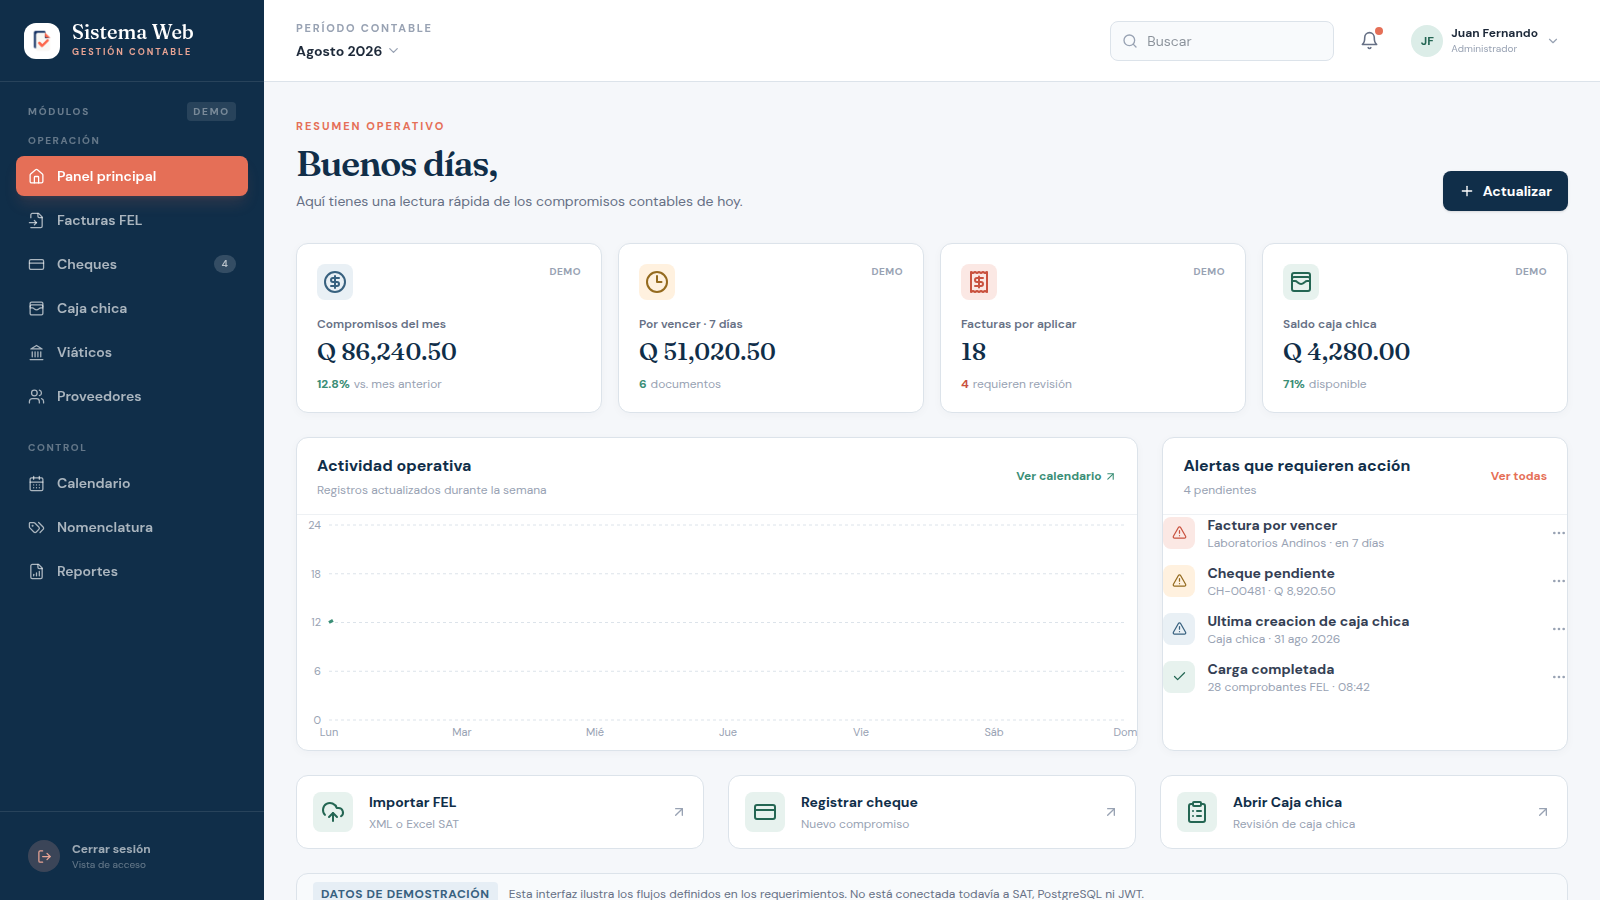
\includegraphics[width=0.96\linewidth]{imagenes/pantalla_02_dashboard.png}
\end{figure}
\begin{table}[H]\centering
\caption{Descripción de Controles del Panel Principal}
\label{tab:3_12_pantalla_dashboard}
\small\setstretch{1.15}
\begin{tabular}{p{0.25\linewidth}p{0.20\linewidth}p{0.20\linewidth}p{0.27\linewidth}}
\toprule
\textbf{Campo o control} & \textbf{Tipo} & \textbf{Valor por defecto} & \textbf{Observación} \\
\midrule
Período contable & Selector & Agosto 2026 & Define el período de consulta. \\
Buscar & Entrada & Vacío & Permite localizar información visible. \\
Indicadores & Tarjetas & Datos demostrativos & Muestran compromisos, vencimientos, facturas y saldo. \\
Alertas & Panel operativo & Pendientes & Presenta actividades que requieren atención. \\
Actualizar & Botón & Activo & Refresca la información del panel. \\
\bottomrule
\end{tabular}
\end{table}


\begin{figure}[H]
    \centering
    \caption{Módulo de Facturas FEL/SAT}
    \label{fig:pantalla_facturas}
    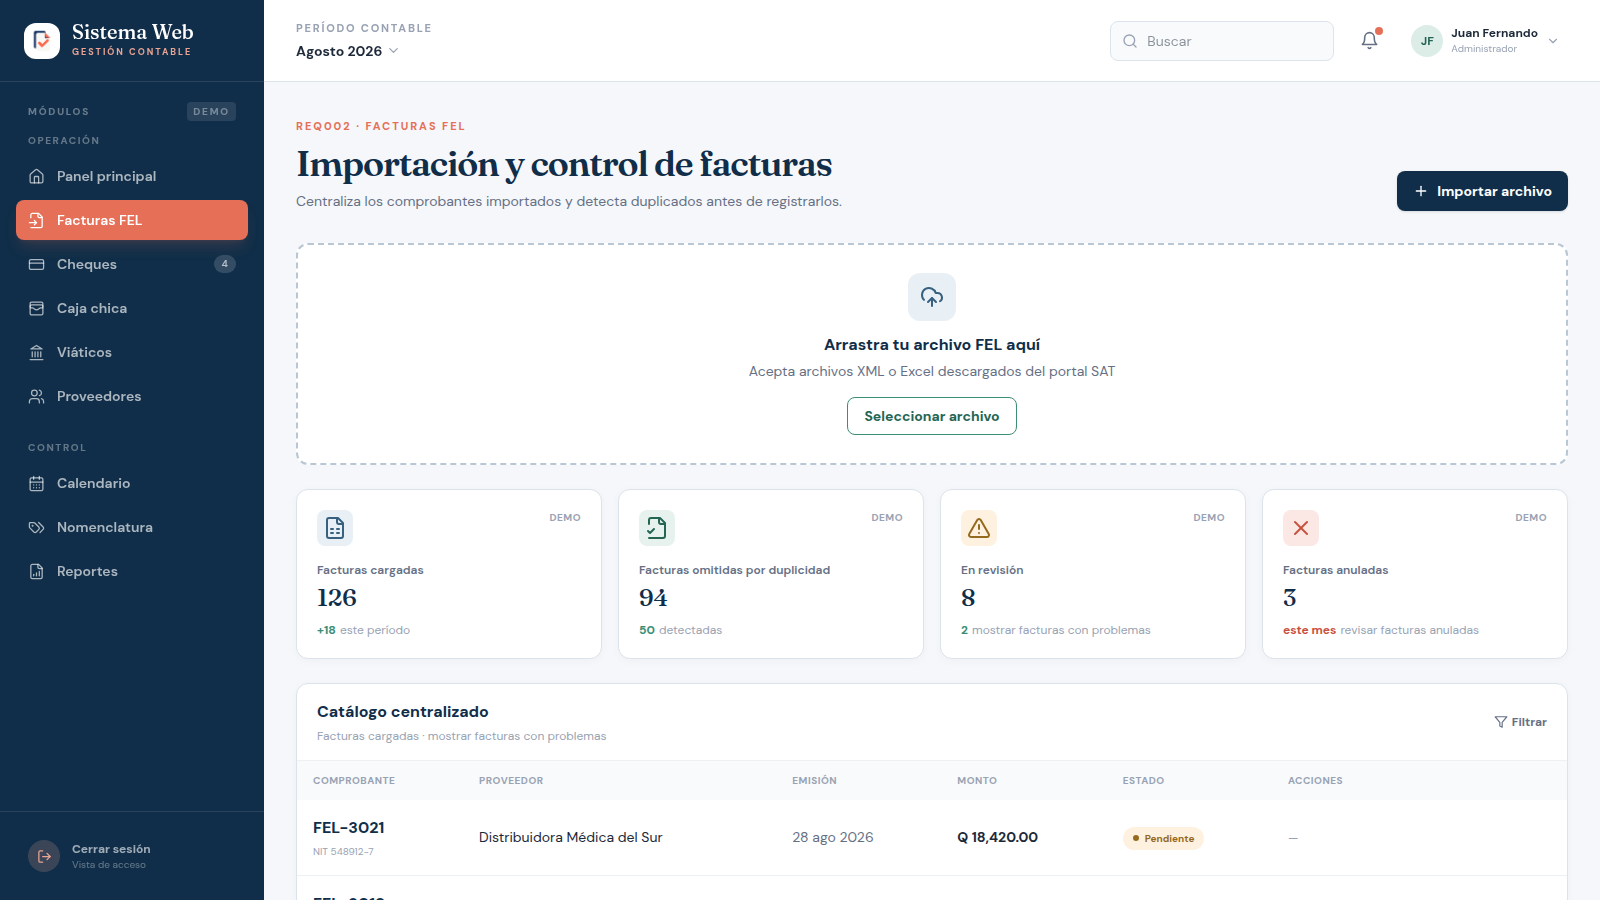
\includegraphics[width=0.96\linewidth]{imagenes/pantalla_03_facturas_fel.png}
\end{figure}
\begin{table}[H]\centering
\caption{Descripción de Controles del Módulo de Facturas FEL/SAT}
\label{tab:3_12_pantalla_facturas}
\small\setstretch{1.15}
\begin{tabular}{p{0.25\linewidth}p{0.20\linewidth}p{0.20\linewidth}p{0.27\linewidth}}
\toprule
\textbf{Campo o control} & \textbf{Tipo} & \textbf{Valor por defecto} & \textbf{Observación} \\
\midrule
Importar archivo & Botón & Activo & Inicia la carga de archivos XML o Excel. \\
Seleccionar archivo & Botón & Sin archivo & Permite elegir el archivo descargado del portal SAT. \\
Catálogo centralizado & Tabla & Registros demostrativos & Muestra comprobante, proveedor, fecha, monto y estado. \\
Editar, Aprobar y Eliminar & Acciones & Según estado & Permiten gestionar una factura autorizada. \\
Filtrar & Control & Sin filtro & Reduce los registros mostrados. \\
\bottomrule
\end{tabular}
\end{table}


\begin{figure}[H]
    \centering
    \caption{Módulo de Cheques postfechados}
    \label{fig:pantalla_cheques}
    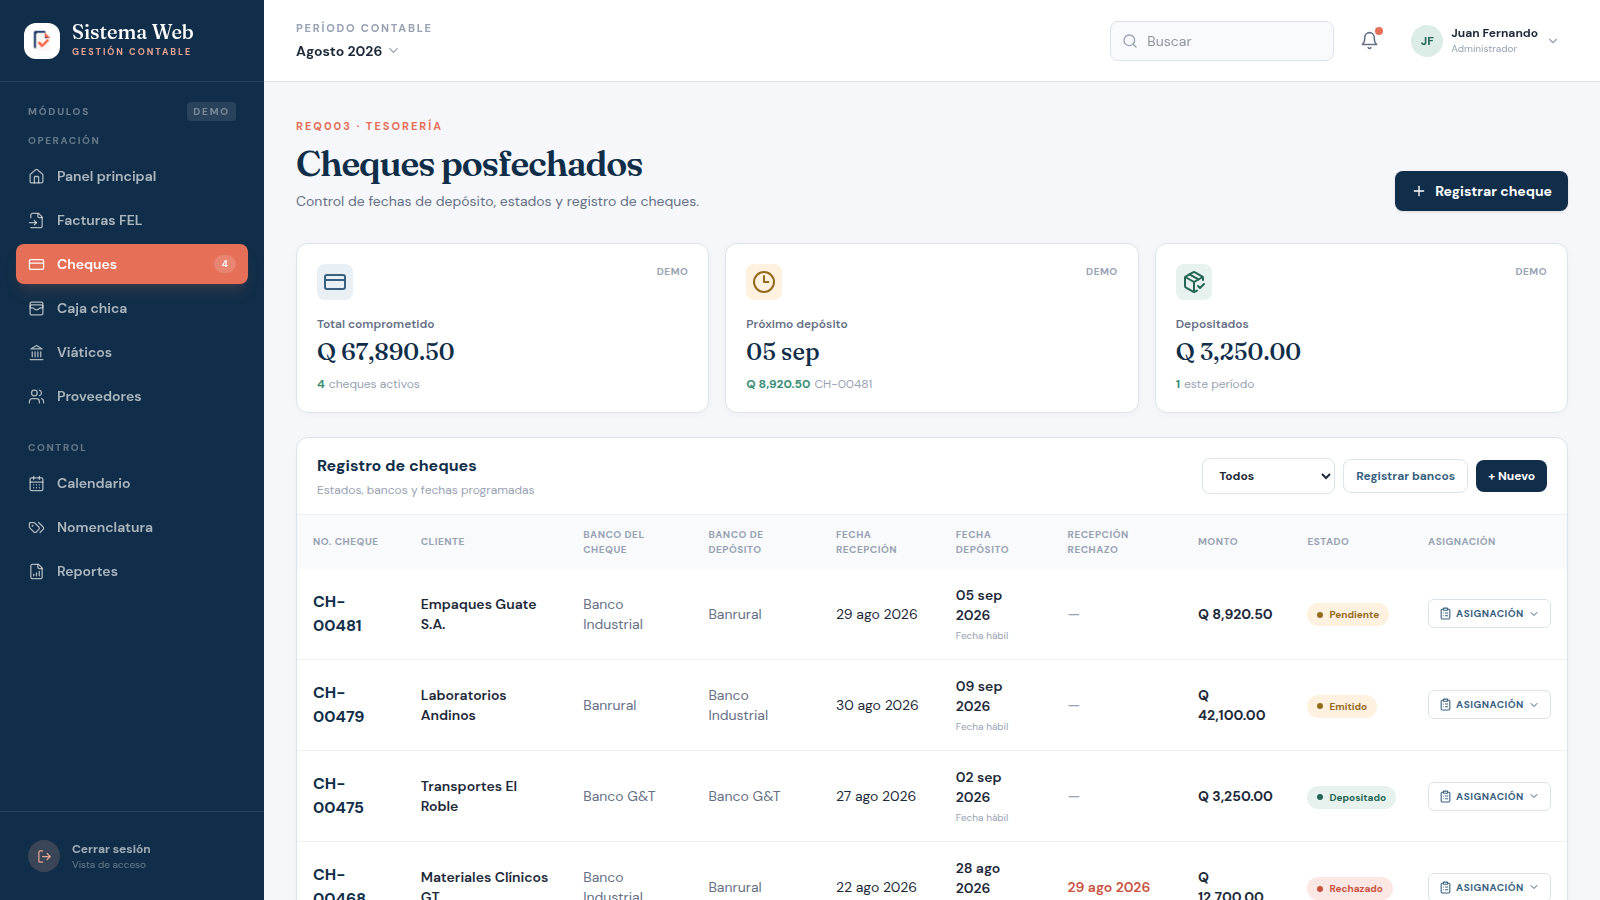
\includegraphics[width=0.96\linewidth]{imagenes/pantalla_04_cheques.png}
\end{figure}
\begin{table}[H]\centering
\caption{Descripción de Controles del Módulo de Cheques}
\label{tab:3_12_pantalla_cheques}
\small\setstretch{1.15}
\begin{tabular}{p{0.25\linewidth}p{0.20\linewidth}p{0.20\linewidth}p{0.27\linewidth}}
\toprule
\textbf{Campo o control} & \textbf{Tipo} & \textbf{Valor por defecto} & \textbf{Observación} \\
\midrule
Estado & Lista desplegable & Todos & Filtra los cheques por estado. \\
Registrar bancos & Botón & Activo & Administra bancos del cheque y de depósito. \\
Nuevo & Botón & Activo & Inicia el registro de un cheque. \\
Registro de cheques & Tabla & Registros demostrativos & Muestra cliente, bancos, fechas, monto y estado. \\
Asignación & Botón desplegable & Disponible & Muestra factura, visitador, recibo y días vencidos. \\
\bottomrule
\end{tabular}
\end{table}


\begin{figure}[H]
    \centering
    \caption{Módulo de Caja chica}
    \label{fig:pantalla_caja}
    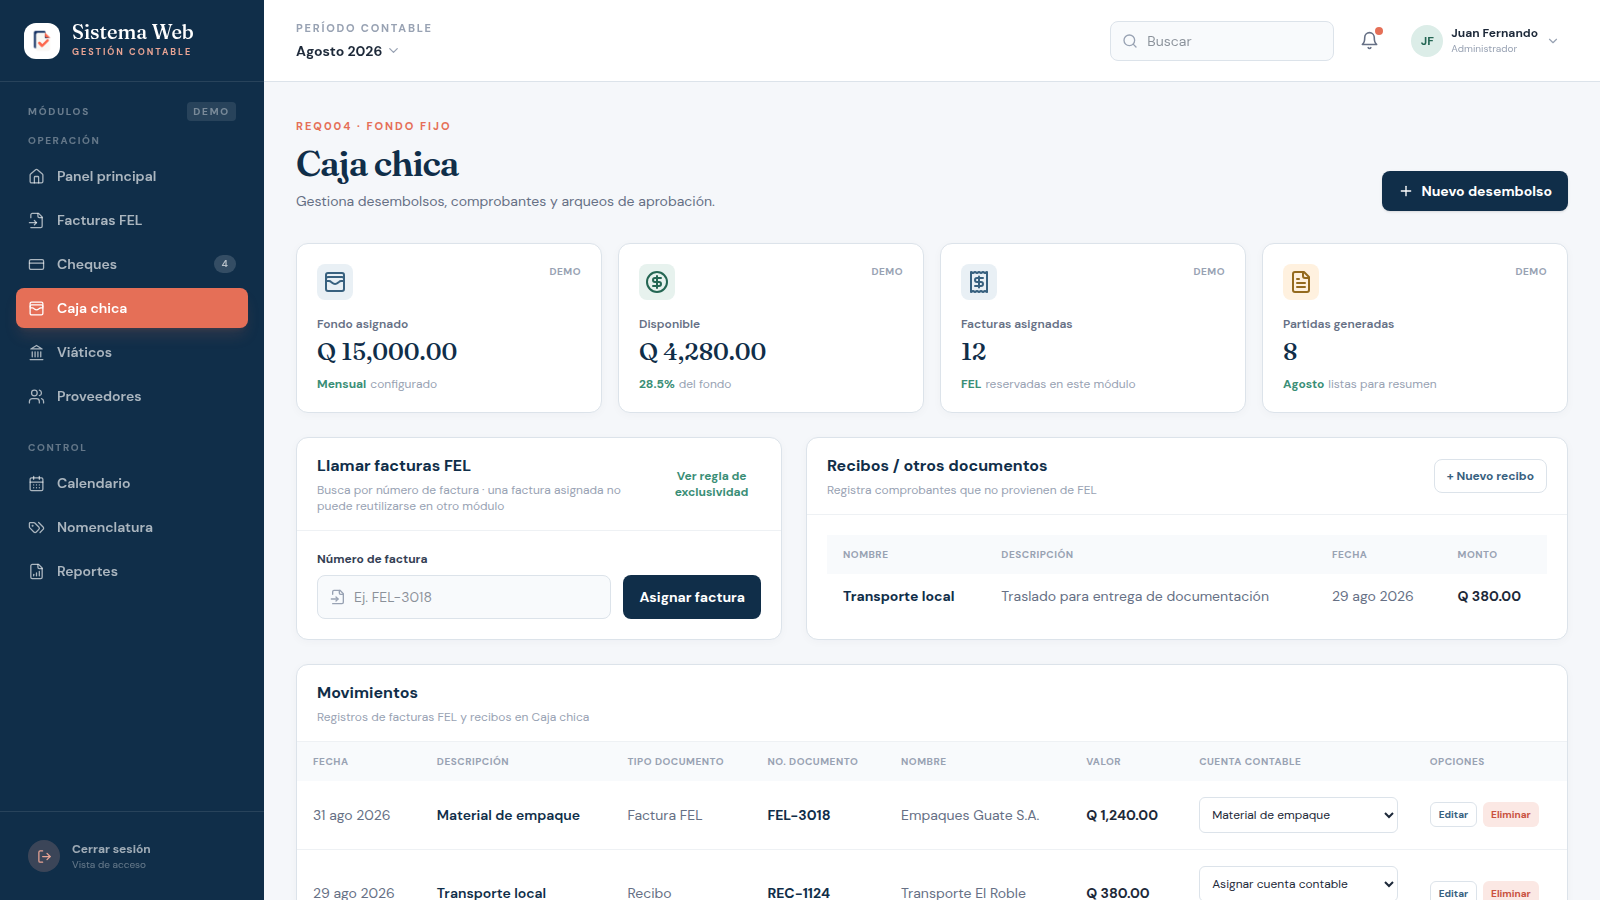
\includegraphics[width=0.96\linewidth]{imagenes/pantalla_05_caja_chica.png}
\end{figure}
\begin{table}[H]\centering
\caption{Descripción de Controles del Módulo de Caja Chica}
\label{tab:3_12_pantalla_caja}
\small\setstretch{1.15}
\begin{tabular}{p{0.25\linewidth}p{0.20\linewidth}p{0.20\linewidth}p{0.27\linewidth}}
\toprule
\textbf{Campo o control} & \textbf{Tipo} & \textbf{Valor por defecto} & \textbf{Observación} \\
\midrule
Número de factura & Entrada & Vacío & Permite llamar una factura FEL por número. \\
Asignar factura & Botón & Activo & Asigna la factura exclusivamente a Caja chica. \\
Nuevo recibo & Botón & Activo & Registra un recibo u otro documento. \\
Cuenta contable & Lista desplegable & Sugerida o manual & Permite seleccionar una cuenta de Nomenclatura. \\
Movimientos & Tabla & Registros demostrativos & Muestra fecha, descripción, documento, nombre, valor y cuenta. \\
Partida contable & Tabla & Debe y Haber & Muestra gastos, IVA y contrapartida. \\
Imprimir resumen & Botón & Activo & Abre el resumen imprimible. \\
\bottomrule
\end{tabular}
\end{table}


\begin{figure}[H]
    \centering
    \caption{Módulo de Viáticos}
    \label{fig:pantalla_viaticos}
    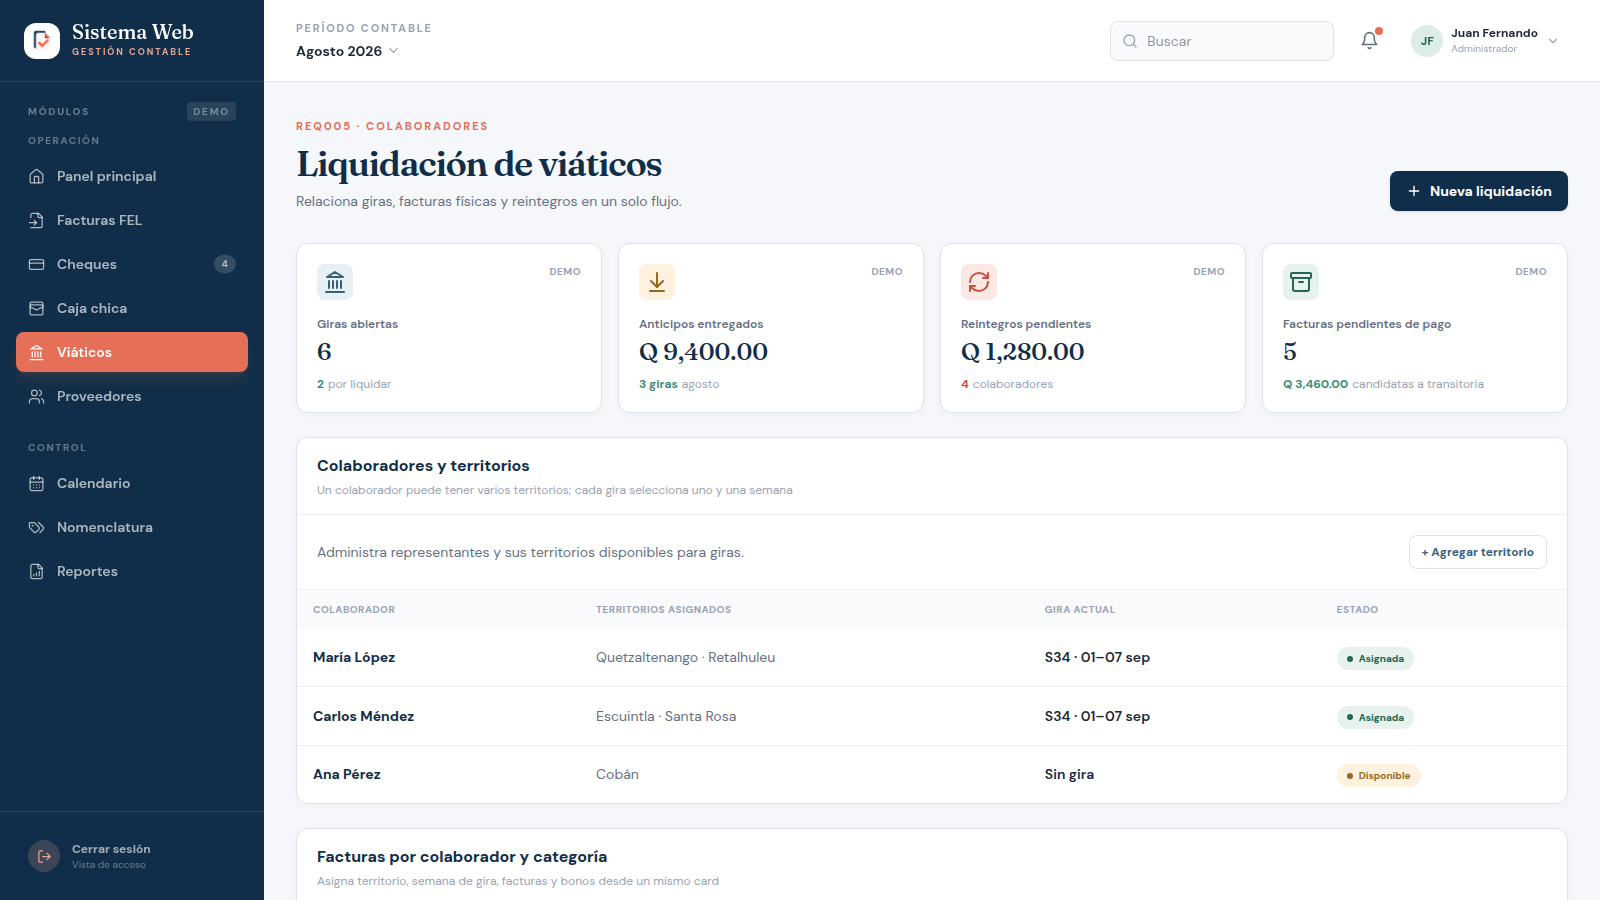
\includegraphics[width=0.96\linewidth]{imagenes/pantalla_06_viaticos.png}
\end{figure}
\begin{table}[H]\centering
\caption{Descripción de Controles del Módulo de Viáticos}
\label{tab:3_12_pantalla_viaticos}
\small\setstretch{1.15}
\begin{tabular}{p{0.25\linewidth}p{0.20\linewidth}p{0.20\linewidth}p{0.27\linewidth}}
\toprule
\textbf{Campo o control} & \textbf{Tipo} & \textbf{Valor por defecto} & \textbf{Observación} \\
\midrule
Agregar territorio & Botón & Activo & Asocia territorios disponibles a colaboradores. \\
Colaborador y gira & Lista desplegable & María López & Selecciona colaborador y territorio. \\
Semana de gira & Lista desplegable & Semana 1 & Selecciona la semana de trabajo. \\
Categoría & Lista desplegable & Viáticos & Permite elegir Viáticos, Movilidad o Actividades. \\
Bonos / otros gastos & Formulario & Vacío & Registra nombre, descripción y monto. \\
Generar partida semanal & Botón & Activo & Genera la partida de la liquidación. \\
Generar cuenta transitoria & Botón & Activo & Agrupa facturas pendientes de pago. \\
\bottomrule
\end{tabular}
\end{table}


\begin{figure}[H]
    \centering
    \caption{Pantalla de asignación de facturas}
    \label{fig:pantalla_asignacion}
    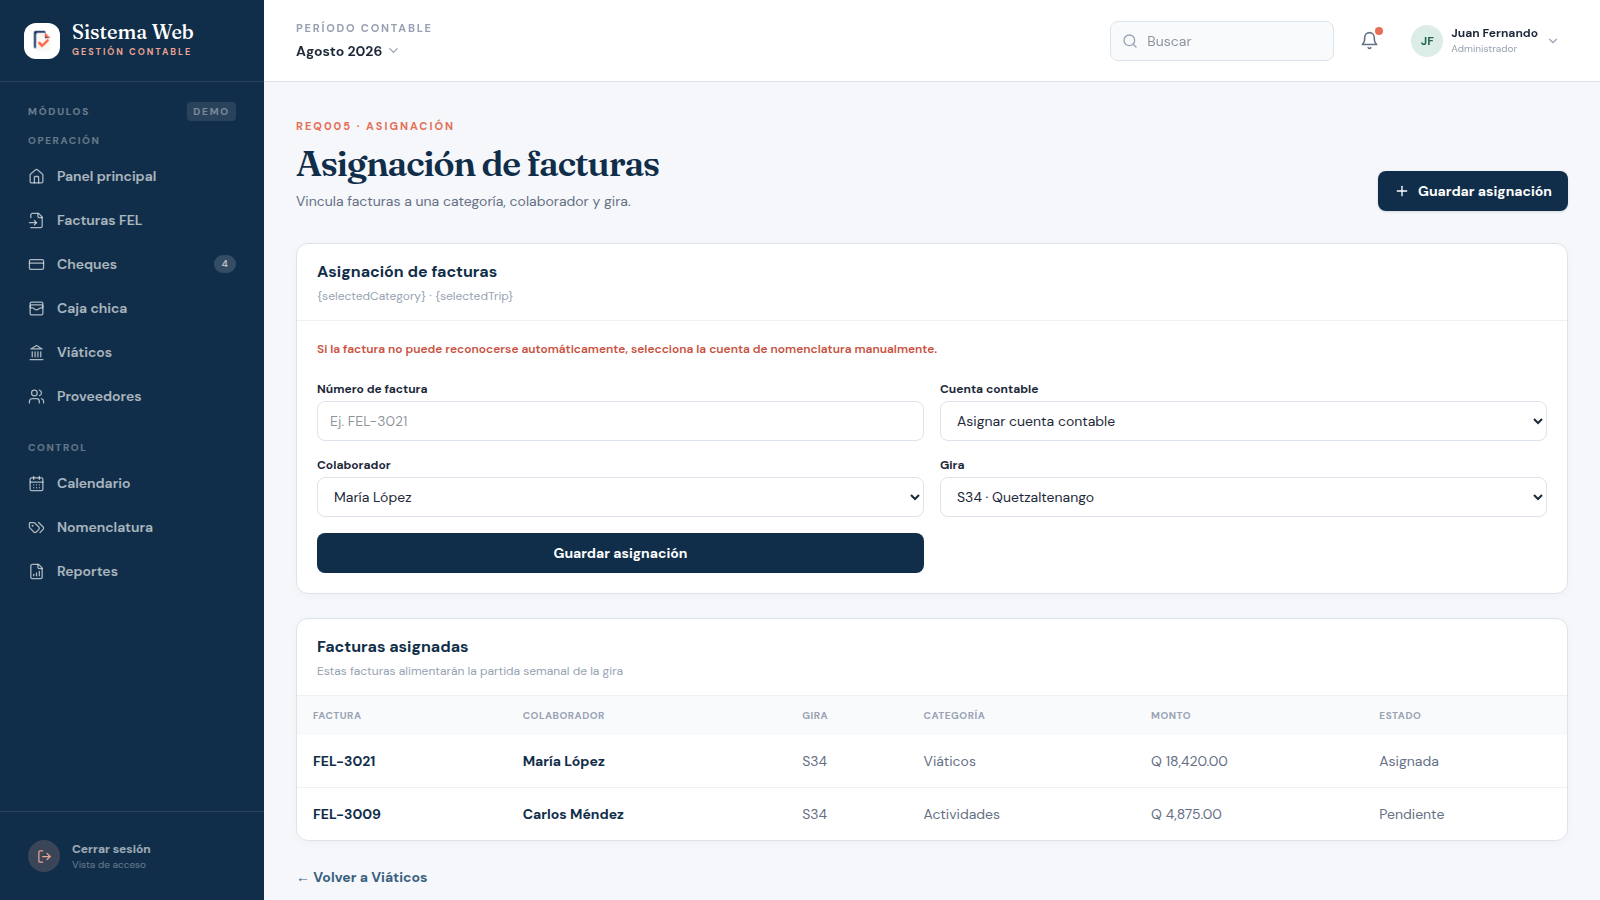
\includegraphics[width=0.96\linewidth]{imagenes/pantalla_07_asignacion_facturas.png}
\end{figure}
\begin{table}[H]\centering
\caption{Descripción de Campos de Asignación de Facturas}
\label{tab:3_12_pantalla_asignacion}
\small\setstretch{1.15}
\begin{tabular}{p{0.25\linewidth}p{0.20\linewidth}p{0.20\linewidth}p{0.27\linewidth}}
\toprule
\textbf{Campo o control} & \textbf{Tipo} & \textbf{Valor por defecto} & \textbf{Observación} \\
\midrule
Número de factura & Entrada & Vacío & Identifica el comprobante que se asignará. \\
Cuenta contable & Lista desplegable & Asignar cuenta contable & Permite seleccionar una cuenta de Nomenclatura. \\
Colaborador & Lista desplegable & María López & Asocia la factura con el colaborador. \\
Gira & Lista desplegable & S34 - Quetzaltenango & Asocia la factura con la gira. \\
Guardar asignación & Botón & Activo & Guarda la relación de factura, cuenta y gira. \\
\bottomrule
\end{tabular}
\end{table}


\begin{figure}[H]
    \centering
    \caption{Módulo de Proveedores}
    \label{fig:pantalla_proveedores}
    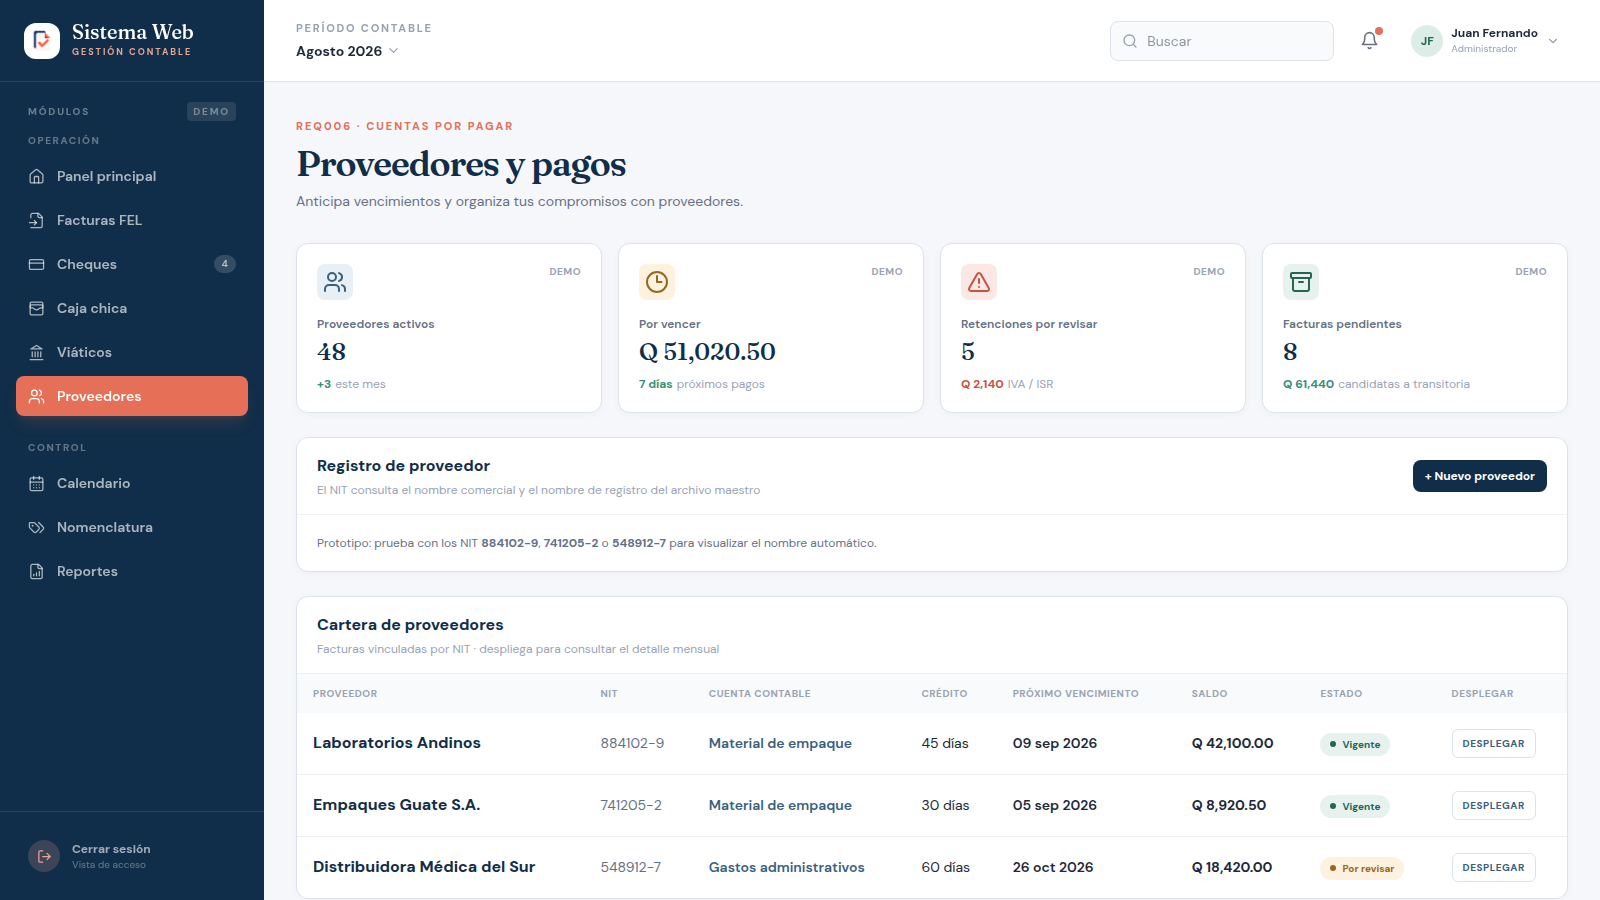
\includegraphics[width=0.96\linewidth]{imagenes/pantalla_08_proveedores.png}
\end{figure}
\begin{table}[H]\centering
\caption{Descripción de Controles del Módulo de Proveedores}
\label{tab:3_12_pantalla_proveedores}
\small\setstretch{1.15}
\begin{tabular}{p{0.25\linewidth}p{0.20\linewidth}p{0.20\linewidth}p{0.27\linewidth}}
\toprule
\textbf{Campo o control} & \textbf{Tipo} & \textbf{Valor por defecto} & \textbf{Observación} \\
\midrule
Nuevo proveedor & Botón & Activo & Inicia el registro por NIT. \\
NIT & Entrada & Vacío & Permite consultar el nombre comercial y de registro. \\
Cuenta contable & Selector & Según proveedor & Asocia la cuenta de Nomenclatura. \\
Cartera de proveedores & Tabla & Registros demostrativos & Muestra crédito, vencimiento, saldo y estado. \\
Desplegar & Botón & Disponible & Muestra las facturas mensuales del proveedor. \\
Generar partida dentro del mes & Botón & Activo & Genera la partida pagadera en el período. \\
Generar partida transitoria & Botón & Activo & Genera la partida de facturas pendientes. \\
\bottomrule
\end{tabular}
\end{table}


\begin{figure}[H]
    \centering
    \caption{Módulo de Calendario}
    \label{fig:pantalla_calendario}
    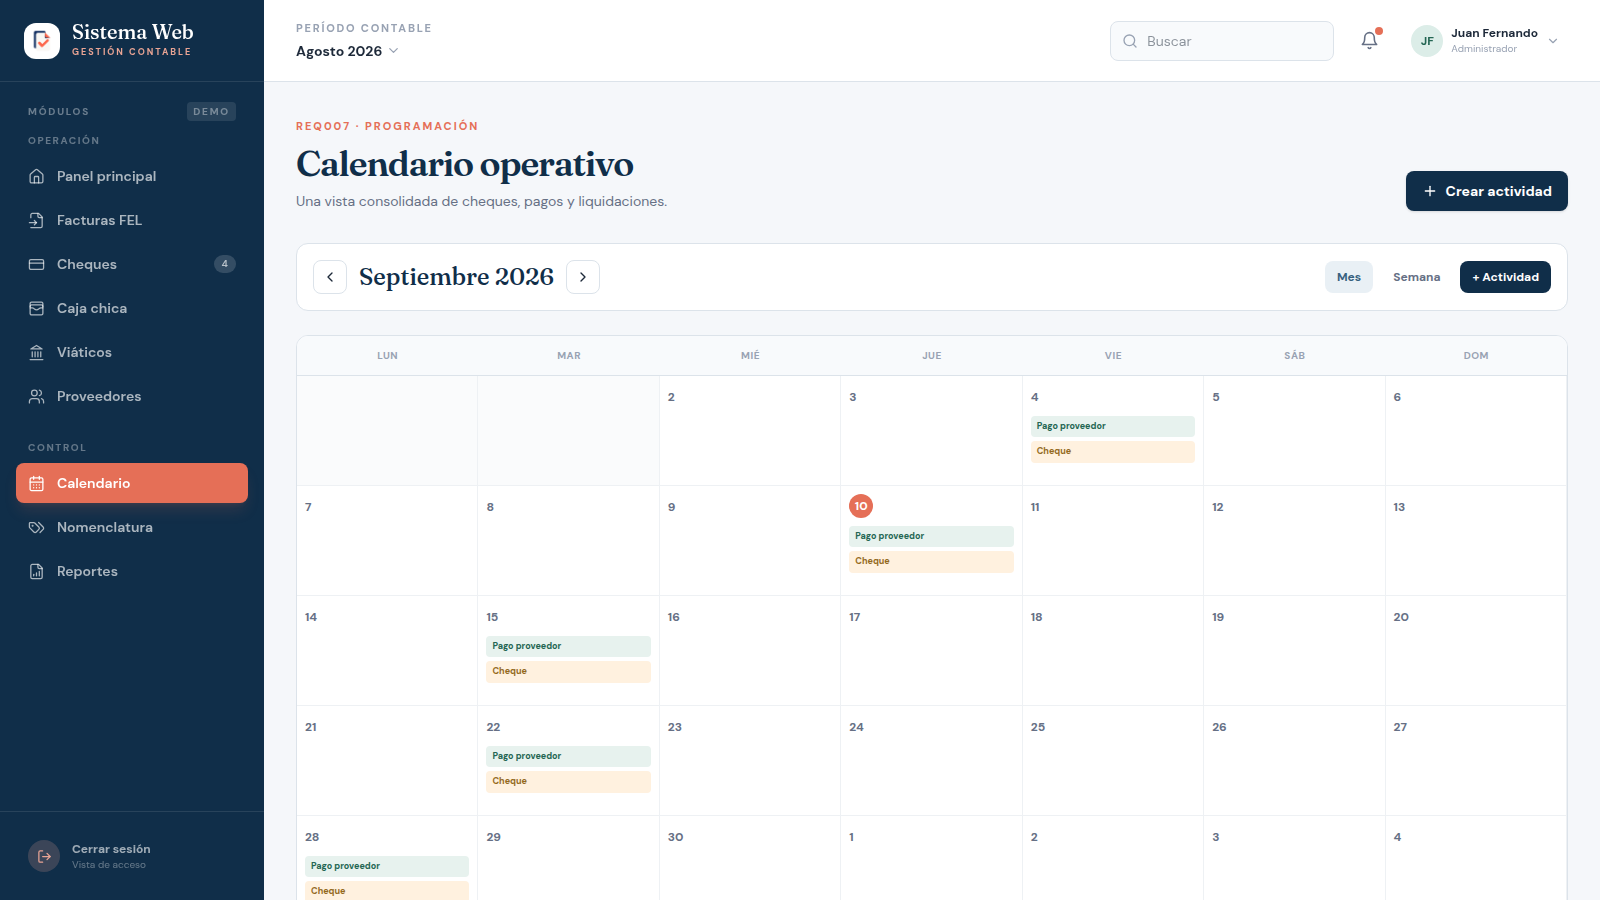
\includegraphics[width=0.96\linewidth]{imagenes/pantalla_09_calendario.png}
\end{figure}
\begin{table}[H]\centering
\caption{Descripción de Controles del Calendario Operativo}
\label{tab:3_12_pantalla_calendario}
\small\setstretch{1.15}
\begin{tabular}{p{0.25\linewidth}p{0.20\linewidth}p{0.20\linewidth}p{0.27\linewidth}}
\toprule
\textbf{Campo o control} & \textbf{Tipo} & \textbf{Valor por defecto} & \textbf{Observación} \\
\midrule
Período mensual & Navegación & Septiembre 2026 & Permite consultar el mes. \\
Anterior y siguiente & Botones & Activos & Cambian el período mostrado. \\
Mes & Selector de vista & Mes & Conserva la vista mensual. \\
Eventos & Calendario & Pagos y cheques & Presenta actividades en la fecha correspondiente. \\
Actividad & Botón & Activo & Permite registrar una actividad. \\
\bottomrule
\end{tabular}
\end{table}


\begin{figure}[H]
    \centering
    \caption{Módulo de Nomenclatura contable}
    \label{fig:pantalla_nomenclatura}
    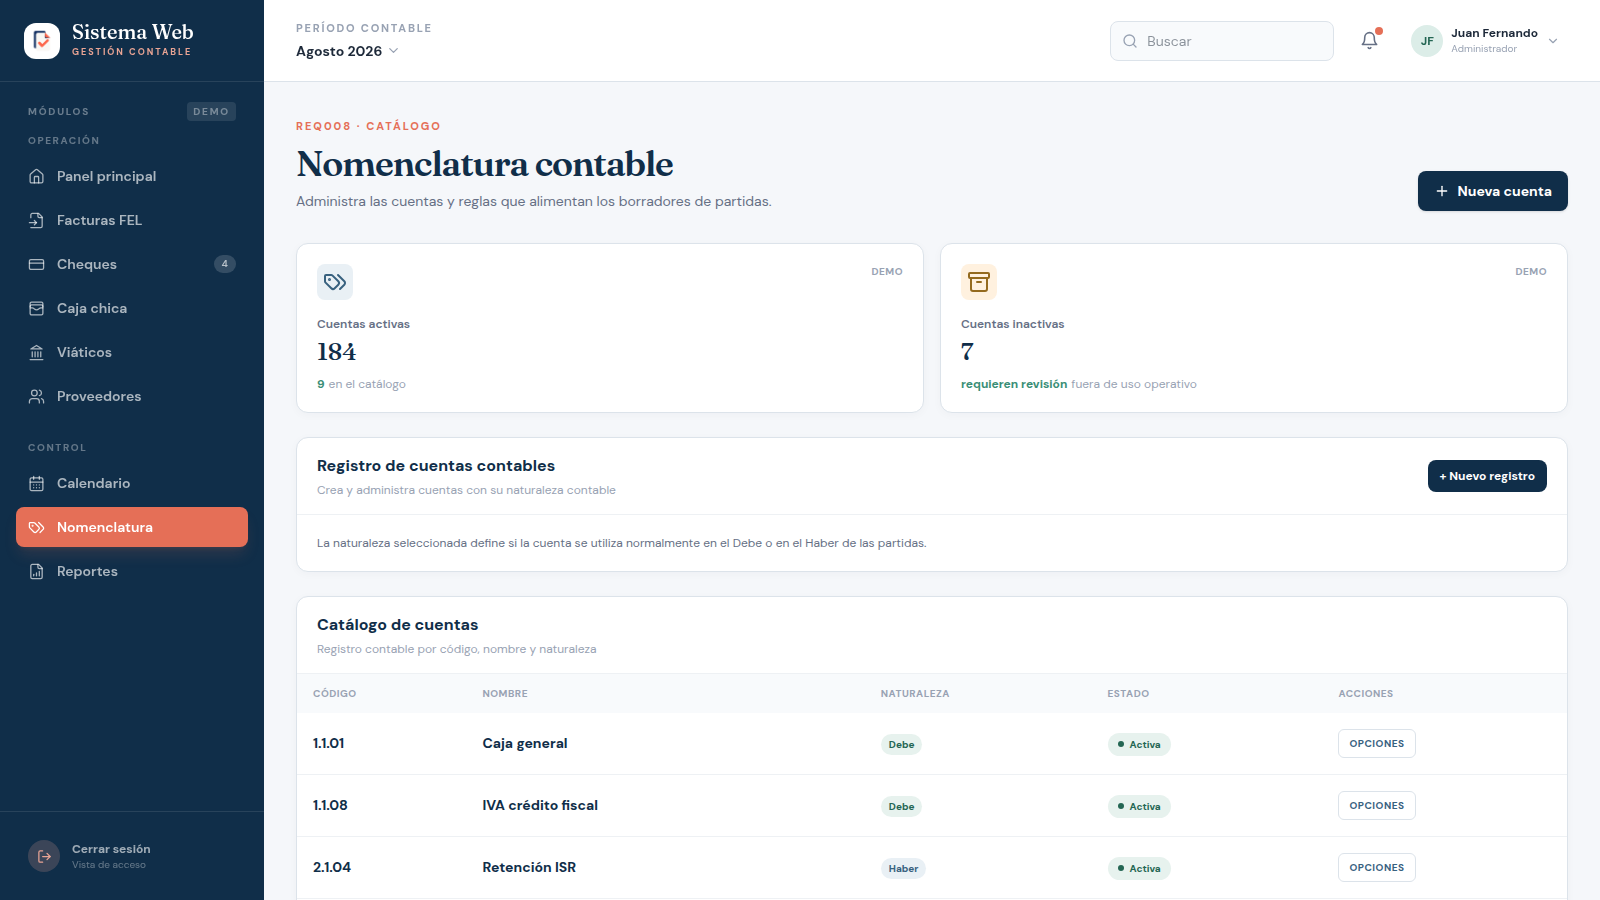
\includegraphics[width=0.96\linewidth]{imagenes/pantalla_10_nomenclatura.png}
\end{figure}
\begin{table}[H]\centering
\caption{Descripción de Controles de Nomenclatura Contable}
\label{tab:3_12_pantalla_nomenclatura}
\small\setstretch{1.15}
\begin{tabular}{p{0.25\linewidth}p{0.20\linewidth}p{0.20\linewidth}p{0.27\linewidth}}
\toprule
\textbf{Campo o control} & \textbf{Tipo} & \textbf{Valor por defecto} & \textbf{Observación} \\
\midrule
Nueva cuenta & Botón & Activo & Inicia la creación de una cuenta. \\
Nuevo registro & Botón & Activo & Abre el formulario de código, nombre y naturaleza. \\
Catálogo de cuentas & Tabla & Registros demostrativos & Muestra código, nombre, naturaleza y estado. \\
Naturaleza & Selector & Debe o Haber & Define la naturaleza contable de la cuenta. \\
Opciones & Botón & Disponible & Permite administrar cada cuenta según permisos. \\
\bottomrule
\end{tabular}
\end{table}


\begin{figure}[H]
    \centering
    \caption{Módulo de Reportes}
    \label{fig:pantalla_reportes}
    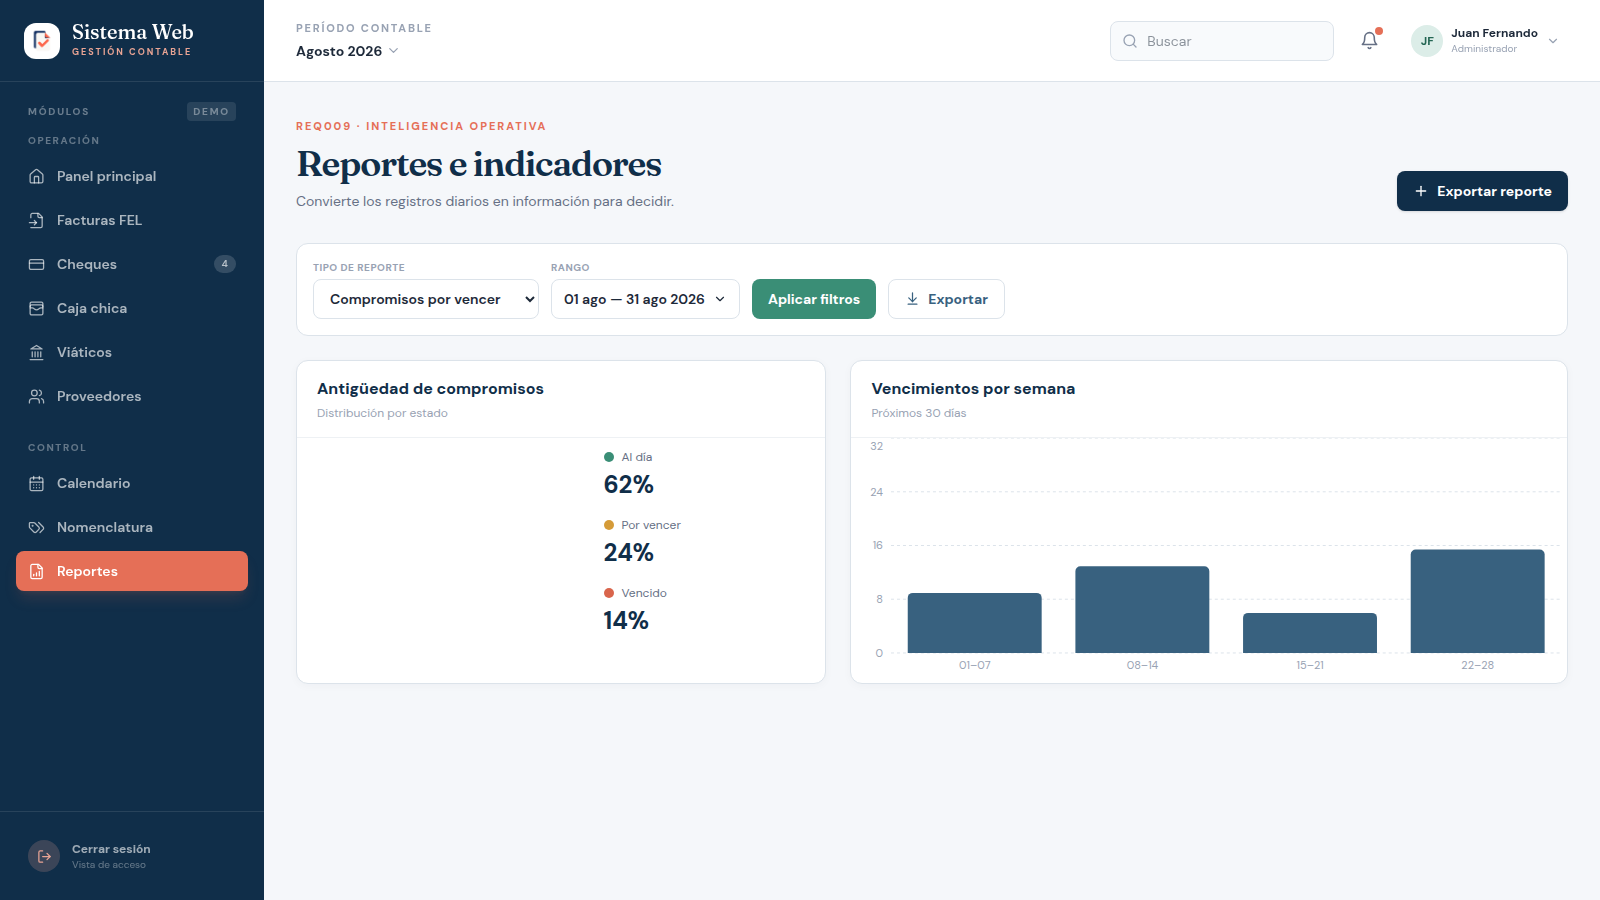
\includegraphics[width=0.96\linewidth]{imagenes/pantalla_11_reportes.png}
\end{figure}
\begin{table}[H]\centering
\caption{Descripción de Controles del Módulo de Reportes}
\label{tab:3_12_pantalla_reportes}
\small\setstretch{1.15}
\begin{tabular}{p{0.25\linewidth}p{0.20\linewidth}p{0.20\linewidth}p{0.27\linewidth}}
\toprule
\textbf{Campo o control} & \textbf{Tipo} & \textbf{Valor por defecto} & \textbf{Observación} \\
\midrule
Tipo de reporte & Lista desplegable & Compromisos por vencer & Selecciona la información que se desea analizar. \\
Rango & Lista desplegable & 01 ago - 31 ago 2026 & Define las fechas de consulta. \\
Aplicar filtros & Botón & Activo & Actualiza gráficos e indicadores. \\
Exportar & Botón & Activo & Prepara el reporte para descarga. \\
\bottomrule
\end{tabular}
\end{table}


\begin{figure}[H]
    \centering
    \caption{Resumen imprimible de Caja chica}
    \label{fig:pantalla_resumen_caja}
    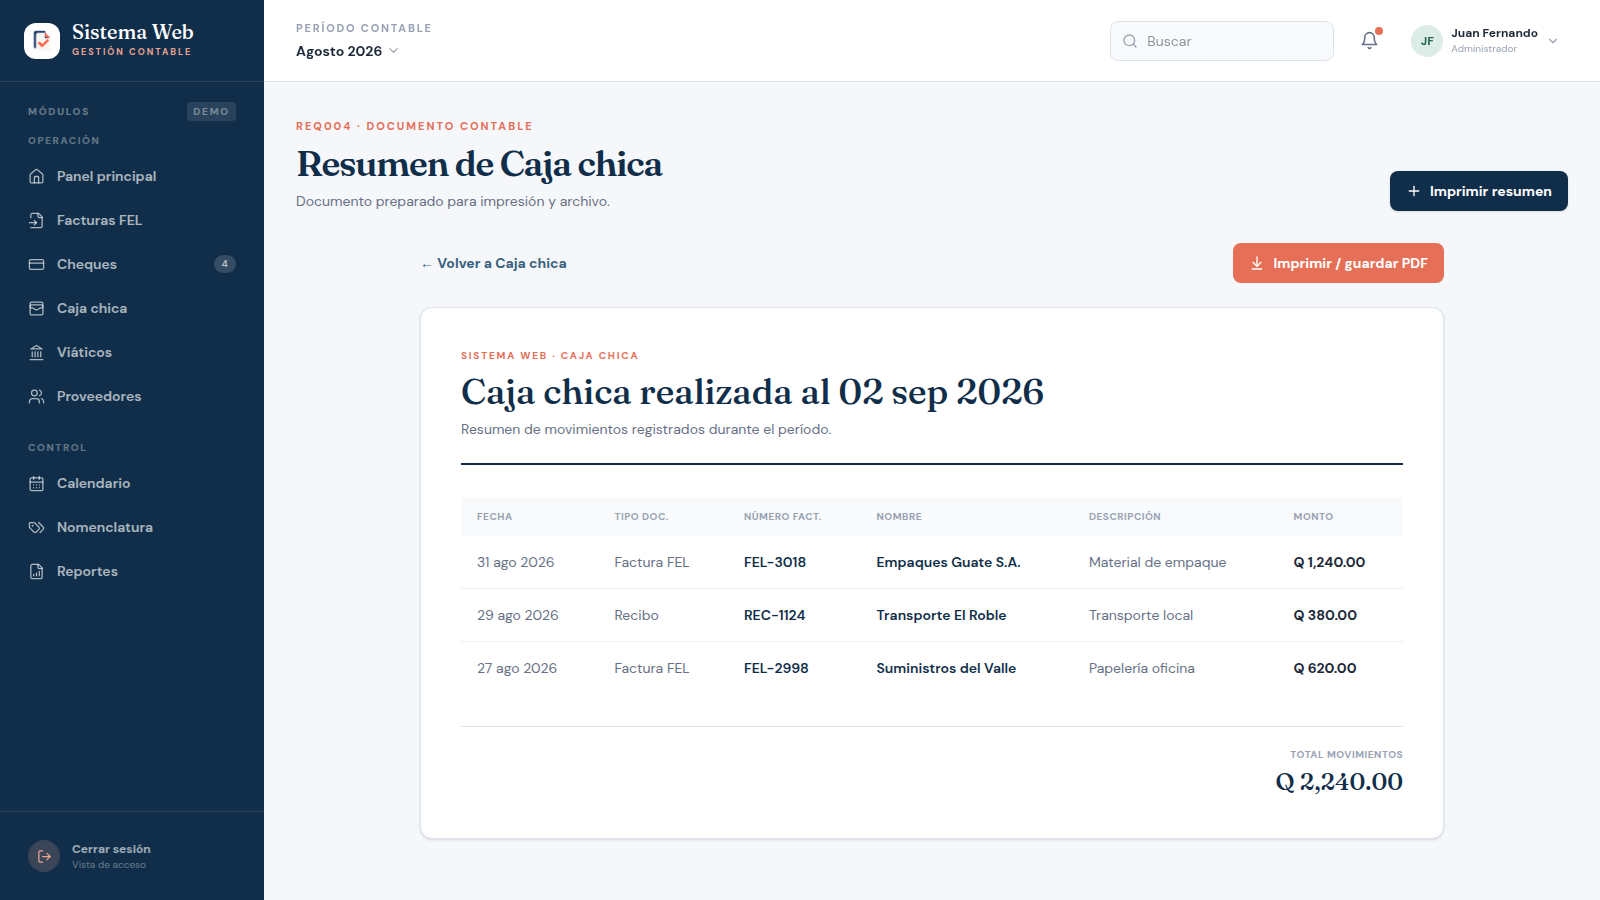
\includegraphics[width=0.96\linewidth]{imagenes/pantalla_12_resumen_caja.png}
\end{figure}
\begin{table}[H]\centering
\caption{Descripción de Controles del Resumen de Caja Chica}
\label{tab:3_12_pantalla_resumen_caja}
\small\setstretch{1.15}
\begin{tabular}{p{0.25\linewidth}p{0.20\linewidth}p{0.20\linewidth}p{0.27\linewidth}}
\toprule
\textbf{Campo o control} & \textbf{Tipo} & \textbf{Valor por defecto} & \textbf{Observación} \\
\midrule
Título y fecha & Encabezado & 02 sep 2026 & Identifica el período del resumen. \\
Imprimir / guardar PDF & Botón & Activo & Abre las opciones de impresión del navegador. \\
Detalle de movimientos & Tabla & Registros demostrativos & Incluye fecha, tipo, número, nombre, descripción y monto. \\
Total de movimientos & Total & Calculado & Permite verificar el importe antes de archivar. \\
\bottomrule
\end{tabular}
\end{table}


\subsection{Arquitectura del Sistema}

El diseño de la aplicación web propuesta se fundamenta en una arquitectura multicapa (n-tier), estructurada bajo una separación lógica de responsabilidades. Este enfoque permite aislar la presentación de la información, el procesamiento de las reglas de negocio y el almacenamiento de los datos, garantizando de esta manera la escalabilidad, el mantenimiento a largo plazo y la seguridad integral de la plataforma financiera.

La Capa de Presentación (Frontend) se desarrolla como una Aplicación de Página Única (SPA, por sus siglas en inglés) utilizando el framework Angular. Esta capa se encarga de ofrecer una interfaz gráfica intuitiva, responsiva y adaptada a las operaciones diarias del área contable. La comunicación con la Capa de Lógica de Negocio (Backend), construida bajo el lenguaje Python, se rige mediante una arquitectura API Restful. Todo el intercambio de información entre el cliente y el servidor se realiza bajo el protocolo seguro HTTPS, utilizando cargas útiles (payloads) en formato JSON y gestionando el control de acceso a través de tokens de autenticación JWT (JSON Web Tokens).

Finalmente, la Capa de Persistencia de Datos recae sobre el sistema gestor de bases de datos relacional PostgreSQL. Esta decisión garantiza el cumplimiento de las propiedades ACID (Atomicidad, Consistencia, Aislamiento y Durabilidad) y la integridad referencial de cada transacción, protegiendo así las partidas de diario y los cálculos contables. Adicionalmente, el modelo contempla un canal de integración externa (Entorno Externo) que permite la carga masiva y el análisis de archivos fiscales (Excel/XML) descargados directamente desde el portal web de la Superintendencia de Administración Tributaria (SAT).

\begin{figure}[H]
    \centering
    \caption{Arquitectura General del Sistema Propuesto}
    \label{fig:arquitectura_sistema}
    \vspace{0.2cm}
    % Se asume que la imagen está en la carpeta de imágenes
    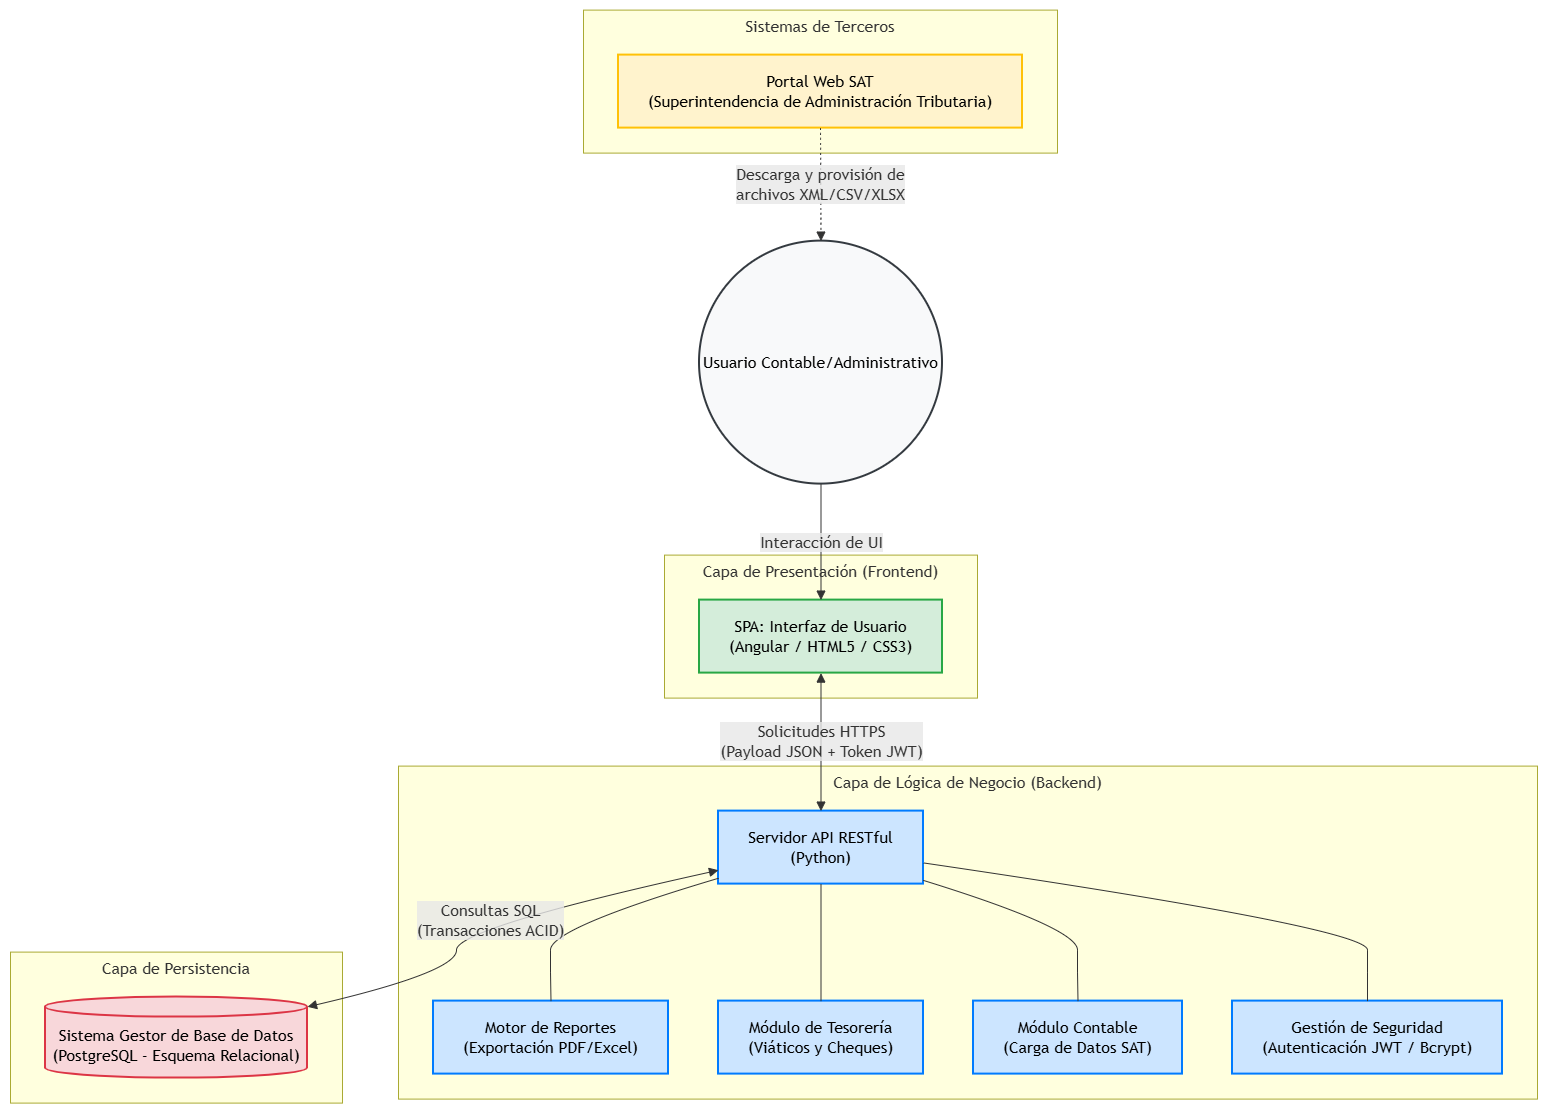
\includegraphics[width=\linewidth]{imagenes/Arquitectura.png}
\end{figure}

\subsection{Factibilidades del Proyecto}

En esta sección se describen las tecnologías y equipos que se requieren para desarrollar e implementar el software, así como la justificación del uso de cada uno. Se detallan las posibilidades y probabilidades con las que el proyecto puede ser llevado a cabo con éxito, evaluando la propuesta desde distintos enfoques técnicos, operativos, económicos, legales y ambientales.

\subsubsection{Factibilidad Técnica}

La factibilidad técnica permitió obtener la información necesaria acerca de si la tecnología requerida para implementar el sistema ya existe en el mercado, así como determinar si se cuenta con las herramientas y el software mínimos necesarios y si estos son accesibles para el desarrollo e implementación del proyecto.

{
\small
\setstretch{1.15}
\setlength{\parindent}{0pt}
\begin{xltabular}{\linewidth}{
    >{\raggedright\arraybackslash}p{4.0cm} 
    >{\raggedright\arraybackslash}p{4.0cm} 
    >{\raggedright\arraybackslash}X
}

    % --- Encabezado de la primera página ---
    \caption{Resumen de Factibilidades de Software} \label{tab:fact_software} \\
    \toprule
    \textbf{Descripción} & \textbf{Motivo} & \textbf{Herramienta Propuesta} \\
    \midrule
    \endfirsthead

    % --- Encabezado en páginas siguientes ---
    \toprule
    \textbf{Descripción} & \textbf{Motivo} & \textbf{Herramienta Propuesta} \\
    \midrule
    \endhead

    % --- Cierre en página intermedia ---
    \bottomrule
    \endfoot

    % --- Cierre final ---
    \bottomrule
    \endlastfoot

    % --- Filas de datos ---
    Lenguaje de Programación & Código fuente del sistema & Python (Backend) / TypeScript (Frontend) \\
    \addlinespace
    IDE & Entorno de desarrollo integrado & Visual Studio Code \\
    \addlinespace
    Framework & Arquitectura del software & Angular (Frontend) / FastAPI (Backend) \\
    \addlinespace
    Formularios e Interfaz & Diseño gráfico de la aplicación & Angular Material / HTML5 / CSS3 \\
    \addlinespace
    Herramienta de Reportes & Generación de documentos PDF & Librerías ReportLab / pdfkit en Python \\
    \addlinespace
    Base de Datos & Almacenamiento relacional de datos & PostgreSQL \\
    \addlinespace
    Gestor de BD & Administración de la base de datos & pgAdmin 4 \\

\end{xltabular}
}

{
\small
\setstretch{1.15}
\setlength{\parindent}{0pt}
\begin{xltabular}{\linewidth}{
    >{\raggedright\arraybackslash}p{4.0cm} 
    >{\raggedright\arraybackslash}X
}

    % --- Encabezado de la primera página ---
    \caption{Resumen de Factibilidades de Hardware} \label{tab:fact_hardware} \\
    \toprule
    \textbf{Descripción} & \textbf{Requisitos Técnicos} \\
    \midrule
    \endfirsthead

    % --- Encabezado en páginas siguientes ---
    \toprule
    \textbf{Descripción} & \textbf{Requisitos Técnicos} \\
    \midrule
    \endhead

    % --- Cierre en página intermedia ---
    \bottomrule
    \endfoot

    % --- Cierre final ---
    \bottomrule
    \endlastfoot

    % --- Filas de datos ---
    Equipo de cómputo & Computadoras con procesador Core i3 o superior, 8 GB de memoria RAM, conexión a internet y navegador web actualizado (Google Chrome o Microsoft Edge). \\
    \addlinespace
    Impresoras & Impresora láser estándar para la generación opcional de comprobantes o reportes físicos contables. \\
    \addlinespace
    Servidor & Servidor local o en la nube (AWS / DigitalOcean) con al menos 4 núcleos, 16 GB de RAM y sistema operativo Linux (Ubuntu Server). \\

\end{xltabular}
}

\subsubsection{Factibilidad Operativa}

El proyecto presenta una factibilidad operativa alta y viable para la distribuidora, sustentada en la evaluación de los siguientes aspectos clave de uso cotidiano:

\paragraph{Aceptación y Usabilidad} El sistema ha sido diseñado con una interfaz clara e intuitiva basada en estándares de Angular Material, lo que reduce significativamente la curva de aprendizaje para el personal administrativo y contable. Para garantizar una transición fluida, se entregará un manual de usuario estructurado y se impartirá una capacitación operativa previa a la puesta en marcha.

\paragraph{Alineación con los Procesos Actuales} La plataforma se integra de manera directa con los flujos de trabajo de la empresa, optimizando el tiempo de ejecución en tareas rutinarias. Al sustituir la digitación manual y las hojas de cálculo dispersas en Excel por la importación masiva de reportes de la SAT y la automatización de partidas contables, se eliminan la duplicidad de funciones y los errores humanos de cálculo sin generar conflictos operativos.

\paragraph{Gestión de la Resistencia al Cambio} La disposición del personal para adoptar la herramienta es positiva, ya que el sistema elimina la carga pesada de tabular manualmente cientos de facturas y llevar registros informales en cuadernos. Al percibir que el software actúa como un asistente que automatiza tareas repetitivas y genera alertas oportunas para pagos y depósitos, la aceptación por parte de los usuarios finales es alta.

\paragraph{Soporte y Mantenimiento Operativo} La distribuidora cuenta con el personal administrativo y contable con el perfil adecuado para la operación diaria de la plataforma. Adicionalmente, se establecerá un periodo de soporte y mantenimiento de 30 días posteriores a la entrega por parte del desarrollador para solventar cualquier eventualidad técnica, asegurando la continuidad del servicio.

\paragraph{Conclusión Operativa} Dado que el sistema satisface de manera directa las necesidades del departamento contable, facilita el trabajo cotidiano de los usuarios y cuenta con el respaldo operativo necesario, se determina que el proyecto es plenamente factible desde la perspectiva operativa.

\subsubsection{Factibilidad Económica}

La factibilidad económica evalúa la relación entre los costos involucrados en el desarrollo del sistema y los beneficios esperados de su uso. Se demuestra que las ventajas y beneficios que se obtendrán con la implementación del software superan con creces los costos asociados a su desarrollo y puesta en funcionamiento.


    \paragraph{Costos de Personal:} No se requiere la contratación de personal adicional para la fase de desarrollo o la operación diaria.
    \paragraph{Costos de Desarrollo:} El sistema es desarrollado por un estudiante de la Universidad Mariano Gálvez de Guatemala como proyecto previo a optar al título de Ingeniero en Sistemas de Información y Ciencias de la Computación, por lo que los costos de desarrollo para la empresa son nulos.
    \paragraph{Costos de Hardware:} La empresa cuenta con los equipos informáticos e infraestructura de red necesarios para operar la aplicación, por lo que no se requiere inversión en nuevo hardware.
    \paragraph{Costos de Software:} El desarrollo emplea herramientas de código abierto con licencias gratuitas, evitando gastos por adquisición de licencias comerciales.


{
\small
\setstretch{1.15}
\setlength{\parindent}{0pt}
\begin{xltabular}{\linewidth}{
    >{\raggedright\arraybackslash}p{3.5cm} 
    >{\raggedright\arraybackslash}X 
    >{\raggedright\arraybackslash}p{2.5cm}
}

    % --- Encabezado de la primera página ---
    \caption{Resumen General de los Costos Reales del Proyecto} \label{tab:costos_reales} \\
    \toprule
    \textbf{Tipo de Costo} & \textbf{Descripción} & \textbf{Valor} \\
    \midrule
    \endfirsthead

    % --- Encabezado en páginas siguientes ---
    \toprule
    \textbf{Tipo de Costo} & \textbf{Descripción} & \textbf{Valor} \\
    \midrule
    \endhead

    % --- Cierre en página intermedia ---
    \bottomrule
    \endfoot

    % --- Cierre final ---
    \bottomrule
    \endlastfoot

    % --- Filas de datos ---
    Costo de Personal & Equipo de trabajo para el desarrollo del proyecto. & Sin Costo \\
    \addlinespace
    Costos de Desarrollo & Análisis, diseño, desarrollo, implementación y pruebas del sistema. & Sin Costo \\
    \addlinespace
    Costos de Hardware & Equipo de cómputo e infraestructura de red existente. & Sin Costo \\
    \addlinespace
    Costos de Software & Licencias de código abierto (PostgreSQL, Angular, Python, FastAPI). & Sin Costo \\
    \addlinespace
    \textbf{Valor Total del Proyecto} & \textbf{Costo de desarrollo asignado al estudiante} & \textbf{Sin Costo} \\

\end{xltabular}
}

\subsubsection{Factibilidad Legal}

Esta sección evalúa el cumplimiento del proyecto respecto a las leyes y regulaciones aplicables en la República de Guatemala, asegurando que el software opere dentro del marco legal tributario, comercial y de propiedad intelectual, evitando posibles sanciones o conflictos futuros.

\paragraph{Licenciamientos de Software}
De acuerdo con la legislación guatemalteca, el software está protegido como una obra intelectual. Las herramientas seleccionadas para el desarrollo (Python, PostgreSQL, Angular y FastAPI) utilizan licencias de código abierto libres y permisivas (como la Licencia MIT), lo que faculta el uso, modificación y despliegue del sistema sin incurrir en infracciones de propiedad intelectual.

\paragraph{Régimen Legal Nacional}
El sistema respalda la validez jurídica e integridad de las operaciones y documentos digitales intercambiados dentro del módulo contable, otorgando certidumbre legal a los registros digitales de cheques, viáticos y liquidaciones de caja chica sin necesidad de trámites físicos en papel.

\paragraph{Acuerdos de Entrega del Proyecto}
El objetivo del acuerdo es entregar a la empresa el Sistema Web documentado, con sus módulos de autenticación, facturas FEL/SAT, cheques, Caja chica, Viáticos, Proveedores, Calendario, Nomenclatura y Reportes. La puesta en operación se realizará conforme al cronograma aprobado por la Universidad y a la disponibilidad operativa de la empresa.

A partir de la entrega se establece un período de 30 días de mantenimiento correctivo y acompañamiento para resolver incidencias, realizar ajustes menores y verificar la estabilidad del sistema. Cualquier ampliación posterior deberá acordarse entre la empresa y el responsable del proyecto.

\paragraph{Consideraciones tributarias y protección de datos}
El módulo FEL procesa y valida archivos XML o Excel conforme a los estándares requeridos por la Superintendencia de Administración Tributaria (SAT). El sistema aplica autenticación y control de acceso por roles para proteger la información financiera de clientes y proveedores.

\subsubsection{Factibilidad Ambiental}

A pesar de que el desarrollo e implementación de software no genera directamente desechos industriales o contaminación física severa, el proyecto ha sido concebido bajo criterios de sostenibilidad y minimización de la huella ecológica.

\paragraph{Digitalización y Reducción del Uso de Papel}
El principal impacto ambiental positivo es la eliminación paulatina de la documentación física. Al automatizar el control de cheques postfechados, la liquidación de viáticos y la conciliación de facturas FEL de la SAT, se reduce drásticamente el consumo de hojas de papel, fotocopias, carpetas e insumos de impresión.

\paragraph{Uso Eficiente de Energía y Servidores Verdes}
Para el alojamiento y despliegue de la aplicación web, se prevé la utilización de proveedores de servicios en la nube (como AWS o Google Cloud) que cuentan con políticas activas de eficiencia energética y el empleo de energías renovables en sus centros de datos.

\paragraph{Programación Ecológica (Green Software)}
Se implementaron buenas prácticas de desarrollo optimizando las consultas a la base de datos y la ejecución de código en el servidor. Esto reduce el consumo innecesario de CPU, memoria y tráfico de red, disminuyendo de manera indirecta el consumo eléctrico de los equipos de cómputo cliente que acceden a la aplicación.

\paragraph{Aprovechamiento de la Infraestructura Existente}
El sistema no requiere la adquisición de nuevos dispositivos electrónicos físicos para la empresa, fomentando la reutilización del equipo de cómputo actual y evitando la generación prematura de basura electrónica (e-waste).

\subsubsection{Análisis de Riesgos del Proyecto}

El desarrollo e implementación del sistema contable implica ciertos riesgos técnicos, operativos y de planificación. Para mitigar su impacto en el éxito del proyecto, se identifican las principales amenazas junto con su nivel de probabilidad, impacto y la estrategia de respuesta correspondiente.

{
\small
\setstretch{1.15}
\setlength{\parindent}{0pt}
\begin{xltabular}{\linewidth}{
    >{\raggedright\arraybackslash}p{2.5cm} 
    >{\raggedright\arraybackslash}p{3.5cm} 
    >{\raggedright\arraybackslash}p{1.8cm} 
    >{\raggedright\arraybackslash}p{1.8cm} 
    >{\raggedright\arraybackslash}X
}

    % --- Encabezado de la primera página ---
    \caption{Matriz de Análisis de Riesgos del Proyecto} \label{tab:analisis_riesgos} \\
    \toprule
    \textbf{Categoría} & \textbf{Riesgo Identificado} & \textbf{Probabilidad} & \textbf{Impacto} & \textbf{Estrategia de Mitigación} \\
    \midrule
    \endfirsthead

    % --- Encabezado en páginas siguientes ---
    \toprule
    \textbf{Categoría} & \textbf{Riesgo Identificado} & \textbf{Probabilidad} & \textbf{Impacto} & \textbf{Estrategia de Mitigación} \\
    \midrule
    \endhead

    % --- Cierre en página intermedia ---
    \bottomrule
    \endfoot

    % --- Cierre final ---
    \bottomrule
    \endlastfoot

    % --- Filas de datos ---
    Técnico & Cambios en la estructura de los archivos XML/Excel emitidos por la SAT. & Media & Alto & Diseñar un módulo de lectura dinámico e implementar validadores de esquemas XML flexibles con manejo claro de excepciones. \\
    \addlinespace
    Técnico & Fallas de conectividad a la base de datos PostgreSQL durante horas pico. & Baja & Alto & Implementar un pool de conexiones optimizado, índices en las tablas contables y respaldos automáticos diarios. \\
    \addlinespace
    Operativo & Resistencia del personal contable a la adopción del nuevo sistema web. & Media & Medio & Involucrar a los usuarios clave en las pruebas iniciales, elaborar un manual claro y brindar capacitaciones guiadas. \\
    \addlinespace
    Seguridad & Accesos no autorizados a la información financiera sensible. & Baja & Alto & Implementar control de acceso basado en roles (RBAC), encriptación de contraseñas y tokens JWT para la sesión de usuario. \\
    \addlinespace
    Planificación & Desfases en las fechas de entrega de los módulos según el cronograma. & Media & Medio & Aplicar el enfoque iterativo e incremental de RUP, evaluando el cumplimiento de hitos clave al finalizar cada fase (Inicio, Elaboración, Construcción y Transición). \\

\end{xltabular}
}
\subsection{Recursos del Proyecto}

Esta sección describe los componentes técnicos, físicos, lógicos y humanos necesarios para el desarrollo, despliegue y funcionamiento óptimo del sistema propuesto.

\subsubsection{Recursos de Hardware}

\paragraph{Servidores} Especificaciones de procesamiento, memoria RAM y capacidad de almacenamiento requerida (por ejemplo, servidor en la nube con 16GB de RAM y 500GB de almacenamiento SSD).

\paragraph{Estaciones de trabajo} Requisitos mínimos para los equipos de los desarrolladores y usuarios administrativos (por ejemplo, Procesador Core i5 o equivalente, 8GB de RAM).

\paragraph{Periféricos} Dispositivos físicos adicionales necesarios para la interacción con el sistema.

\subsubsection{Recursos de Software}

\paragraph{Sistemas Operativos} Plataformas sobre las cuales se ejecutará el sistema y los entornos de desarrollo (por ejemplo, Windows 10/11, distribuciones Linux, o sistemas móviles).

\paragraph{Gestores de Bases de Datos} Motor de base de datos seleccionado para el almacenamiento seguro de la información (por ejemplo, MySQL, PostgreSQL o SQL Server).

\paragraph{Lenguajes y Frameworks} Tecnologías principales utilizadas en el backend y frontend para la construcción del software.

\paragraph{Herramientas de Terceros} APIs, pasarelas de pago o librerías externas que el sistema consume para su funcionamiento.

\subsubsection{Recursos de Red y Comunicaciones}

\paragraph{Conectividad} Requisitos de ancho de banda y acceso a internet continuo para garantizar la disponibilidad del sistema alojado en la red.

\paragraph{Seguridad} Implementación de certificados SSL/TLS para el cifrado de datos en tránsito y configuración de firewalls para la protección de la infraestructura.

\subsubsection{Recursos Humanos}

\paragraph{Equipo Técnico} Roles indispensables para la creación y mantenimiento del proyecto, como desarrolladores de software, analistas de sistemas y administradores de bases de datos.

\paragraph{Usuarios del Sistema} Personal que operará la plataforma y que requerirá capacitación básica para el manejo de las interfaces.




\subsection{Cronograma de Actividades del Proyecto}

En la siguiente figura se presenta el diagrama de Gantt, el cual detalla la planificación y el tiempo estimado para cada una de las fases y actividades del proyecto.

\begin{landscape}

\begin{figure}[H]
    \centering
      \caption{Diagrama de Gantt.}
    \label{fig:diagrama_gantt}
    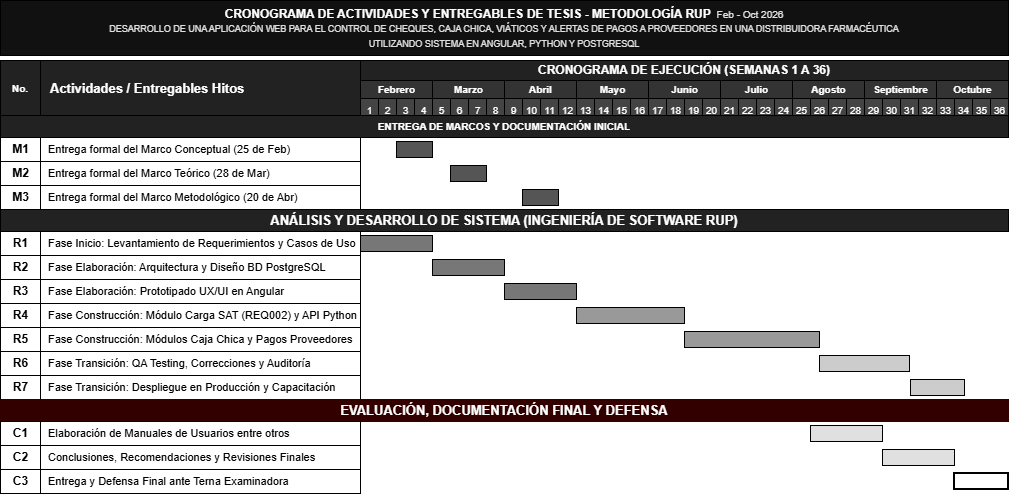
\includegraphics[width=\linewidth]{imagenes/image7.png}

\end{figure}

\end{landscape}